\section{Continuum mechanics}

Continuum mechanics allows to define general equations of motion for a wide range of phenomena from liquids to deformable solids. 
In this section, we propose a progressive introduction to the basics of continuum mechanics and provide details about the physical models used in the following chapters. 
Firstly, we describe how to formulate general equations of motion and we present the different concepts and numerical tools used to solve them.
Secondly, we present a constitutive law for fluid mechanics leading to Navier-Stokes equations and we detail their discretization using the Smoothed-Particle Hydrodynamics (SPH) model that will serve as background for our contribution in Chapter~\ref{chap:arps}.
Finally, we present a constitutive law for solid mechanics which allows to simulate elastic solids and we detail the discretization of the equations of motion using the frame-based model that we use in Chapter~\ref{chap:cutting}.
If the reader looks for a wider presentation of the existing deformable models in Computer Graphics, we suggest the survey of Nealen et al.~\cite{Nealen2006}.
%\subsection{Notation}
%
%We will use the following notations throughout this manuscript.
%\begin{table}[!h]
%\begin{tabular}{ll}
%$t$ & time \\
%$m$ &  mass \\
%$\rho$ & mass density \\
%$\mathbf{n}$ & normal \\
%$\mathbf{x}$ & position \\
%$\mathbf{v}$ & velocity \\
%$\mathbf{f}$ & total forces \\
%$\mathbf{f}_{int}$ & internal forces \\
%$\mathbf{f}_{ext}$ & external forces \\
%$F$ & Deformation gradient \\
%$\epsilon$ & Strain tensor \\
%$\sigma$ & Stress tensor \\
%$\Psi$ & Energy density \\
%\end{tabular}
%\end{table}

\subsection{Equations of motion}

The equations of motion describe the behavior of an object over time.
They are generally derived from conservation laws such as mass and momentum conservation. 
A constitutive law is also used to depict the intrinsic behavior of the simulated object.
The remainder of this section first describes the conservation laws used to formulate general equations of motion.
Then we detail the concepts and numerical tools used to solve these equations.

\subsubsection{Conservation of mass}

The conservation of mass states that, whatever the physical material which is studied, mass cannot be created or destroyed.
More precisely, if we look at a small volume of the simulation domain, the variation of mass in that volume should be equal to the flux of mass going through its border.
In Figure~\ref{fig:massConservation}, we illustrate this law with the example of a glass of water.
At a time $t_{1}$, the mass of the water should be equal to its mass at time $t_{0}$ plus the mass of the inflow and minus the mass of the outflow which occurred between $t_{0}$ and $t_{1}$.
\begin{figure}[!h]
	\centering
	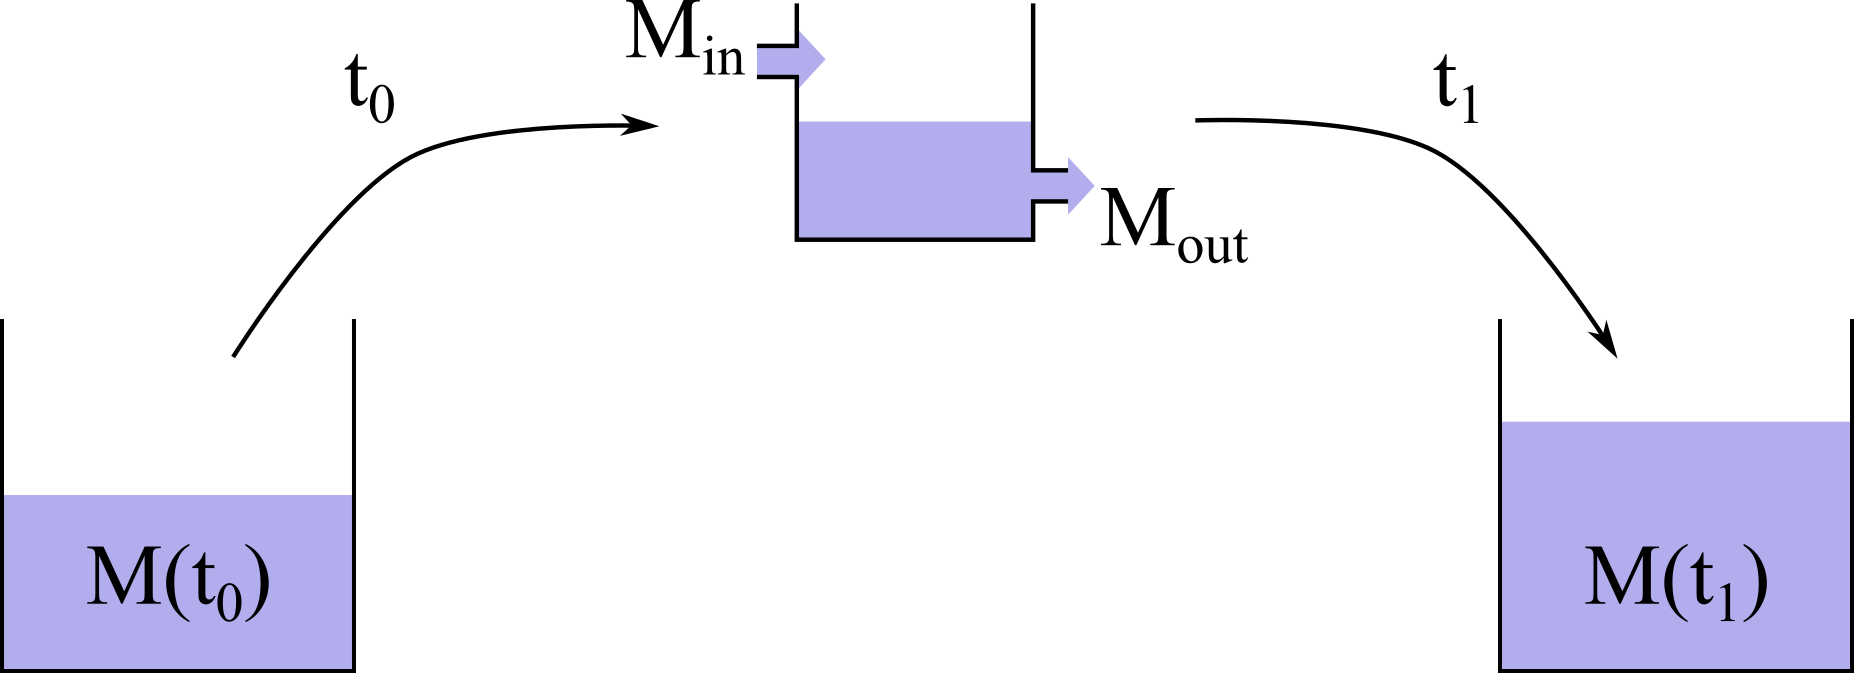
\includegraphics[width=\linewidth]{images/continuum_mechanics/massConservation.png}
	\caption[STAR mechanics: Mass conservation]{\label{fig:massConservation} Mass conservation. $M(t_{1}) = M(t_{0}) + M_{in} - M_{out}$}
\end{figure}
\\
Mathematically, we can write the conservation of mass as
\begin{equation}
    \label{eq:massConservation}
    \displaystyle 
    \frac{d}{dt}\left( \int_{\mathcal{V}} \rho(t,\mathbf{x}) dv \right)
    =
    - \int_{\mathcal{\partial V}}\rho(t,\mathbf{x})\mathbf{v}(t,\mathbf{x}) \cdot \mathbf{n}(\mathbf{x}) ds
\end{equation}
where
\begin{itemize}
	\item $\rho(t,\mathbf{x})$ is the density at a point $\mathbf{x}$ and at a time $t$.
	\item $\mathbf{v}(t,\mathbf{x})$ is the velocity at a point $\mathbf{x}$ and at a time $t$.
	\item $\mathcal{V}$ is a small volume of the simulation domain $\Omega$.
	\item $\mathcal{\partial V}$ is the border of $\mathcal{V}$.
	\item $\mathbf{n}(\mathbf{x})$ is the normal of $\mathcal{V}$ on a point $\mathbf{x}$ of $\partial\mathcal{V}$.
\end{itemize}
This formulation involves an integral over the volume and its boundary.
When numerically solving this equation, it is simpler not to have to make the distinction between a small element of $\mathcal{V}$ and a small element of $\partial \mathcal{V}$.
By using Stokes' theorem, we have
\begin{equation}
\displaystyle 
\int_{\partial \mathcal{V}} \rho \mathbf{v} \cdot \mathbf{n} ds =
\int_{\mathcal{V}} \nabla \cdot \left( \rho \mathbf{v} \right) dv
\end{equation}
and we can rewrite Equation~(\ref{eq:massConservation}) as a single integral over $\mathcal{V}$
\begin{equation}
\label{eq:volumetricMassConservation}
\displaystyle 
\int_{\mathcal{V}} 
\left( \frac{\partial \rho}{\partial t} + \nabla \cdot \left( \rho  \mathbf{v} \right) \right) dv = 0
\end{equation}

\subsubsection{Conservation of momentum}

The conservation of momentum is implied by Newton's second law which states that the forces applied on an object result into an acceleration which is inversely proportional to the mass of the object.
Figure~\ref{fig:momentumConservation} illustrates this law in the case of two balls on which a same force is applied.
The acceleration induced by the force is more important for the small ball which has a mass less important than the big ball.
\begin{figure}[!h]
\centering
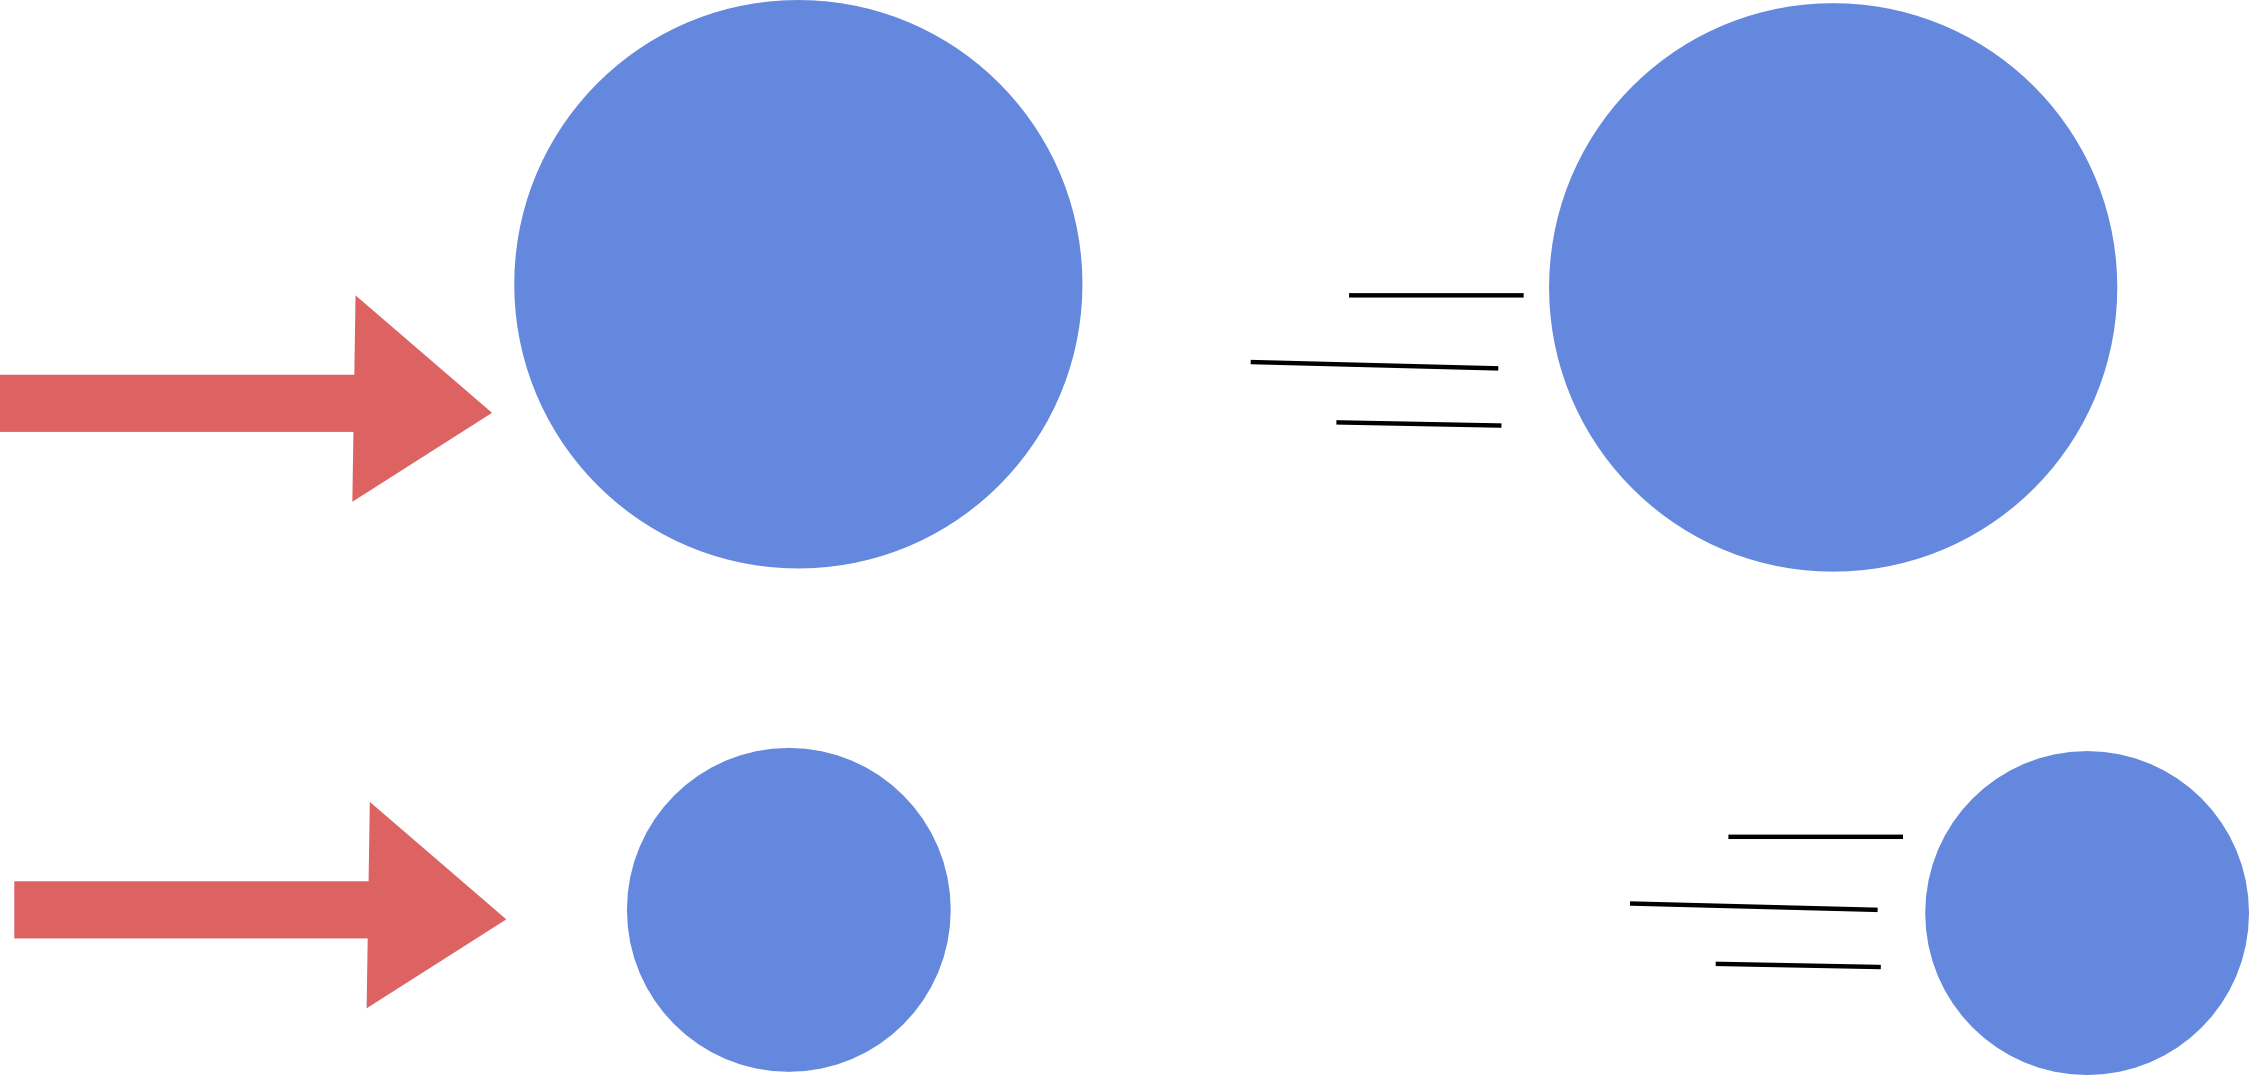
\includegraphics[width=\linewidth]{images/continuum_mechanics/momentumConservation.png}
\caption[STAR mechanics: Momentum conservation]{\label{fig:momentumConservation} Momentum conservation. The same force $\mathbf{f}$ is applied on two balls. The resulting acceleration is inversely proportional to their mass.}
\end{figure}
\\
Mathematically, this law can be written as
\begin{equation}
\displaystyle 
\int_{\mathcal{V}} 
\rho(t,\mathbf{x})\mathbf{a}(t,\mathbf{x}) dv 
= 
\int_{\mathcal{V}} \mathbf{f}(t,\mathbf{x}) dv
\end{equation}
where
\begin{itemize}
	\item $\mathbf{a}(t,\mathbf{x})$ is the acceleration at a point $\mathbf{x}$ and at a time $t$.
		\item $\mathbf{f}(t,\mathbf{x})$ is the force applied on a point $\mathbf{x}$ and at a time $t$.
\end{itemize}
By performing a Taylor-Young expansion on the acceleration, we can re-write the momentum conservation as
\begin{equation}
\label{eq:momentumConservation}
\displaystyle 
\int_{\mathcal{V}} 
\rho(t,\mathbf{x}) \left( \frac{\partial\mathbf{v}}{\partial t} + \mathbf{v} \cdot \nabla \mathbf{v} \right)(t,\mathbf{x}) dv 
= 
\int_{\mathcal{V}} \mathbf{f}(t,\mathbf{x}) dv
\end{equation}
Two kind of forces are generally applied on an object, the \emph{external} forces and the \emph{internal} forces.
External forces describe the action of the surrounding environment on the object. 
The simplest example is the weight, i.e. the force applied by the constant gravity $\mathbf{g}$ on the object:
\begin{equation}
\displaystyle \int_{\mathcal{V}} \mathbf{f}_{ext}(t,\mathbf{x})dv = \int_{\mathcal{V}} \rho(t,\mathbf{x}) \mathbf{g} dv
\end{equation}
Internal forces describe the reaction of the object to an external deformation.
Generally, they are defined by using a stress tensor $\sigma(t,\mathbf{x})$ as 
\begin{equation}
\displaystyle 
\int_{\mathcal{V}} \mathbf{f}_{int}(t,\mathbf{x}) dv 
= \int_{\partial \mathcal{V}} \sigma(t,\mathbf{x}) \mathbf{n}(\mathbf{x}) ds
\end{equation}
Basically, the stress relates the deformation of the object to its material properties by using a constitutive law.
A constitutive law is specific to the phenomena which is simulated.
In Section~\ref{subsec:fluidMechanics} and Section~\ref{subsec:solidMechanics}, we will respectively describe the most common constitutive laws for incompressible fluids and solids.
For a detailed and intuitive definition of the stress tensor we refer the reader to the \emph{SIGGRAPH} course about real-time physics~\cite{Muller2008} by M\"{u}ller et al.
\\
Same as for the conservation of mass, we can use Stokes' theorem to get a single integral over $\mathcal{V}$,
\begin{equation}
\displaystyle 
\int_{\mathcal{\partial V}} \sigma \mathbf{n} ds =
\int_{\mathcal{V}} \nabla \cdot \sigma dv
\end{equation}
and we can rewrite Equation~(\ref{eq:momentumConservation}) as
\begin{equation}
\label{eq:volumetricMomentumConservation}
\displaystyle
\int_{\mathcal{V}} 
\left( 
\rho \left( \frac{\partial\mathbf{v}}{\partial t} + \mathbf{v} \cdot \nabla \mathbf{v} \right)
- \nabla \cdot \sigma - \rho \mathbf{g}  \right) dv = 0
\end{equation}

\subsubsection{Eulerian vs. Lagrangian formulations}

Eulerian and Lagrangian formulations are two different ways of interpreting the equations of motion.
To understand the key difference, we take the example of the simulation of a river and use Figure~\ref{fig:EulerianVsLagrangian} to illustrate it.
Let us suppose that we want to measure fluid properties such as velocity, density or temperature of the river.
A first possibility would be to measure it at a fixed location, similarly to a buoy that would remain at the same spot and measures data at regular intervals of time. This is the Eulerian viewpoint. A second possibility is to measure it along a path that would follow the flow of the river, similarly to an object floating on the river or a particle of water moving accordingly to the flow. This is the Lagrangian viewpoint.
\begin{figure}[!ht]
	\centering
	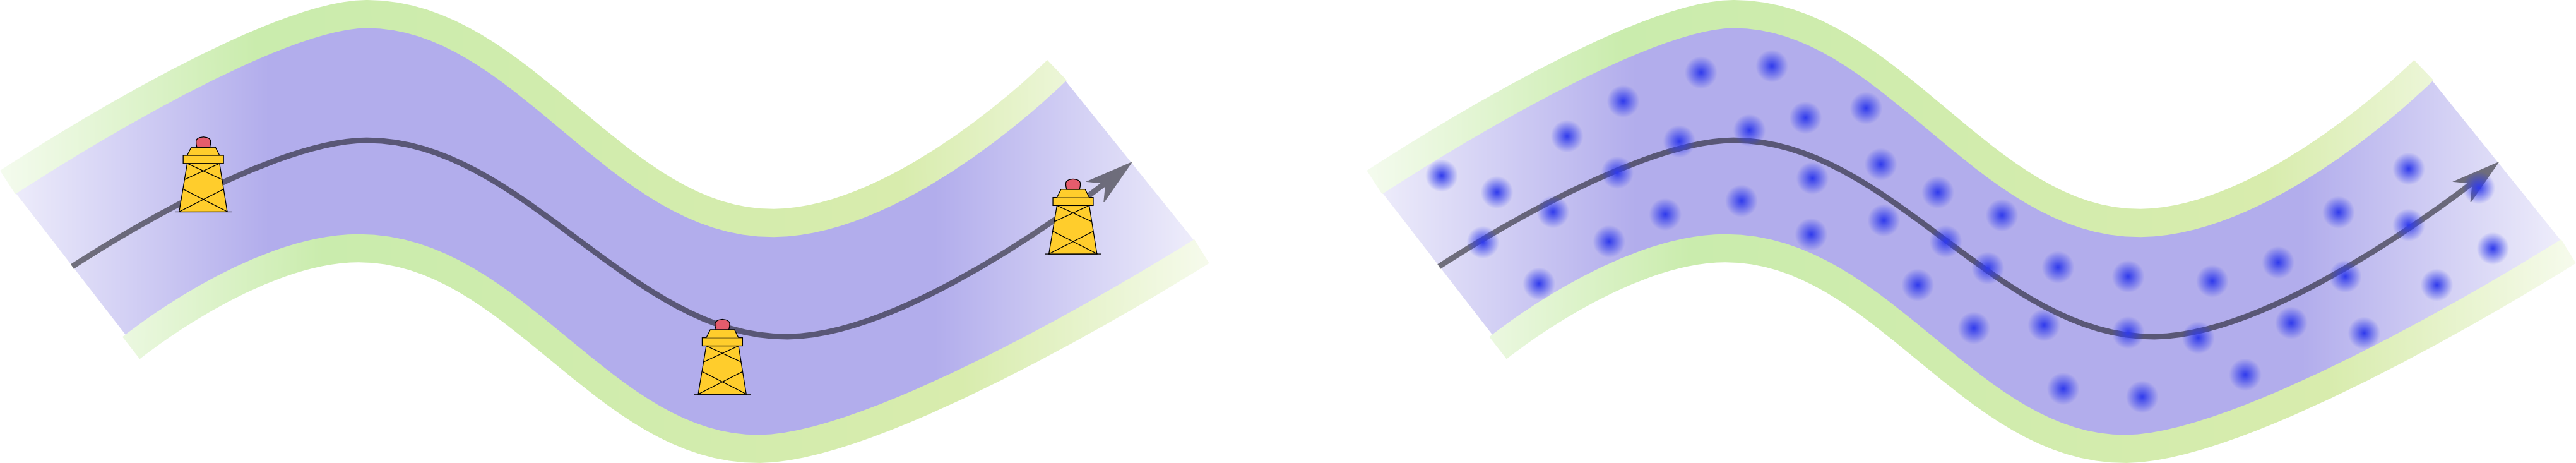
\includegraphics[width=\linewidth]{images/continuum_mechanics/eulerianVsLagrangian.png}
	\caption[STAR mechanics: Eulerian vs. Lagrangian]{\label{fig:EulerianVsLagrangian} Eulerian vs. Lagrangian viewpoint. On the left, buoys are put at fixed positions on a river and measure properties such as velocity, temperature, etc. The Eulerian approach takes a similar approach. On the right, we represent the river with particles of water which follows the flow of the river and carry properties with them. This is similar to the Lagrangian viewpoint.}
\end{figure}
Equation~\ref{eq:volumetricMassConservation} and Equation~\ref{eq:volumetricMomentumConservation} are described for fixed locations. Put together, they define the equations of motion from an Eulerian viewpoint.
\begin{equation}
\label{eq:eulerianMotionEquation}
\left\lbrace
\begin{array}{l}
\displaystyle 
\int_{\mathcal{V}} 
\left( 
\rho \left( \frac{\partial\mathbf{v}}{\partial t} + \mathbf{v} \cdot \nabla \mathbf{v} \right)
- \nabla \cdot \sigma - \rho \mathbf{g}  \right) dv = 0 
\\ \\
\displaystyle
\int_{\mathcal{V}} 
\left( \frac{\partial \rho}{\partial t} + \nabla \cdot \left( \rho  \mathbf{v} \right) \right) dv = 0
\end{array}
\right.
\end{equation}
In order to adopt the Lagrangian viewpoint, let us suppose that the fluid properties are carried by particle and that $q(t,\mathbf{x})$ denote one of this property at a time $t$ for a particle which is at a position $\mathbf{x}$. 
If we want to compute the derivative of $q$ for the particle at position $\mathbf{x}$, we have to use the total derivative:
\begin{equation}
\label{eq:totalDerivative}
\frac{dq(t,\mathbf{x})}{dt} = 
\frac{\partial q}{\partial t}\cdot\frac{dt}{dt} + \frac{\partial q}{\partial \mathbf{x}} \cdot \frac{d\mathbf{x}}{dt} 
= \frac{\partial q}{\partial t}(t,\mathbf{x}) + \left(\nabla q(t,\mathbf{x}) \cdot \mathbf{v}\right)(t,\mathbf{x})
\end{equation}
In Equation~(\ref{eq:volumetricMomentumConservation}) which describes the momentum conservation, we can directly use Equation~(\ref{eq:totalDerivative}) to adopt a Lagrangian viewpoint. 
For the mass conservation described in Equation~(\ref{eq:volumetricMassConservation}), we first need to develop the divergence of the product between density and velocity and then Equation~(\ref{eq:totalDerivative}) can be used.
Finally, we can write the equations of motion from a Lagrangian viewpoint as
\begin{equation}
\label{eq:lagrangianMotionEquation}
\left\lbrace
\begin{array}{l}
\displaystyle 
\int_{\mathcal{V}} 
\left( 
\rho \frac{d\mathbf{v}}{dt}
- \nabla \cdot \sigma - \rho \mathbf{g}  \right) dv = 0 
\\ \\
\displaystyle
\int_{\mathcal{V}} 
\left( \frac{d\rho}{dt} + \rho \nabla \cdot \mathbf{v} \right) dv = 0
\end{array}
\right.
\end{equation}
As the deformable models used in Chapter~\ref{chap:arps} and Chapter~\ref{chap:cutting} are used to solve Lagrangian equations of motion, we will keep Equation~\ref{eq:lagrangianMotionEquation} in the following sections.
%In Lagrangian simulations, conservation of mass is guaranteed by assuming that the mass of the particles are constant over time. In this context, numerically solving of equation~(\ref{eq:lagrangianMassConservation}) can be omitted. It is worth to notice that in Lagrangian liquid simulations, conservation of the mass does not imply incompressibility. To insure the latter, equation~(\ref{eq:lagrangianMassConservation}) needs to be revisited and integrated within the numerical solver. An approach to enforce incompressibility was recently proposed for SPH simulations by Bender and Koschier~\cite{Bender2015}.
\subsubsection{Numerical solution}

Once the equations of motion are stated, they are discretized in space and time in order to be numerically solved.

\paragraph{Spatial discretization}
The spatial discretization consists in approximating the object to simulate using a finite number of samples. 
These samples carry the \emph{degrees of freedom} used to numerically solve the equations of motion.
Then, by using an \emph{interpolation method}, it is possible to approximate continuous quantities such as position, velocity, density and so on, at any location on the domain. 
Finally, a \emph{quadrature rule} is needed in order to integrate these quantities over the domain. 
These are the main components for solving the equations of motion:
degrees of freedom, an interpolation method and a quadrature rule for the numerical integration over the simulation domain.
\\ \\
There are multiple possibilities for these components: It is crucial to choose them based on the goals of the simulation, What do we want to measure ? How will boundaries be represented ? Will any topological changes occur ? Are there restrictions in terms of computational or memory cost ? In the following we briefly introduce the most commonly used solutions in Computer Graphics.

\subparagraph{Degrees of freedom}
In Eulerian simulation, velocities are the most common independent degrees of freedom while Lagrangian simulations generally use positions and velocities. 
We can also mention the use of affine frames to capture translations, rotations and shearing. They are used in the frame-based model which will be detailed in Section~\ref{subsubsec:framebased}.
\\ 
Usually, we distinguish two types of sampling of the degrees of freedom: mesh-based and mesh-less (see Figure~\ref{fig:discretization}).
\begin{figure}[!h]
	\centering
	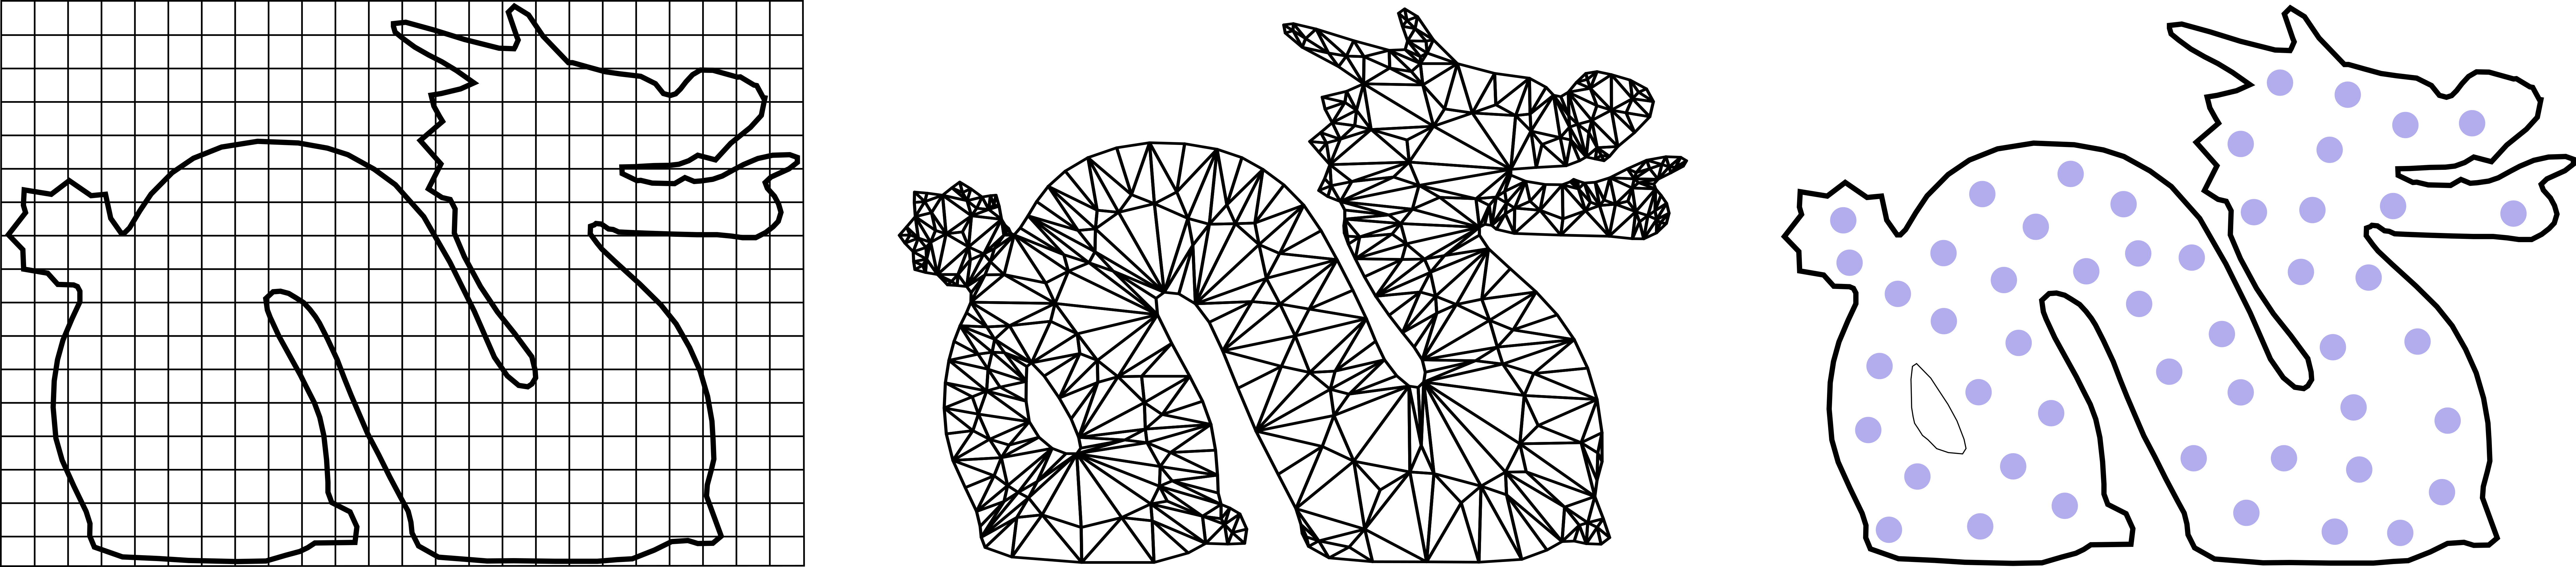
\includegraphics[width=\linewidth]{images/continuum_mechanics/discretization.png}
	\caption[STAR mechanics: Discretization]{\label{fig:discretization} On the left a grid discretization, commonly used in Eulerian simulations. In the middle an unstructured mesh discretization, commonly used in mesh-based Lagrangian simulations. On the right, a point-based discretization, commonly used in mesh-less Lagrangian simulations.}
\end{figure}
\\
In mesh-based methods, the vertices of a mesh are used to sample the degrees of freedom. For instance, Eulerian simulations usually use a cartesian grid which allows to accurately compute derivatives. 
In contrast, Lagrangian simulations are mostly based on unstructured triangular meshes which allows to handle complex boundaries.
In mesh-less methods, the samples are uniformly distributed over the domain. Depending on the simulated phenomena, the structure may be quasi-nonexistent which brings a lot of flexibility. For fluids, the neighborhood of the samples will change every time whereas for elastic solids their neighborhood will remain the same as long as the object does not undergo topological changes such as fracture or cutting.
Of course, each of these samplings can benefit from adaptivity. We will detail the different possibilities of spatial adaptivity in Chapter~\ref{chap:starAdaptivity}.

\subparagraph{Interpolation}
Interpolation is used to approximate the physical quantities over the domain such as density, displacement, pressure and so on. 
In Computer Graphics, we can distinguish three major interpolation methods: polynomial interpolation, Moving Least Squares (MLS) and Smoothed-Particles Hydrodynamics (SPH) interpolation. 
For each of them, different weights are used, as illustrated in Figure~\ref{fig:shapefunction}. The weights are also called \emph{shape functions}, they can be seen as the region of influence of a sample.
\begin{figure}[!h]
	\centering
	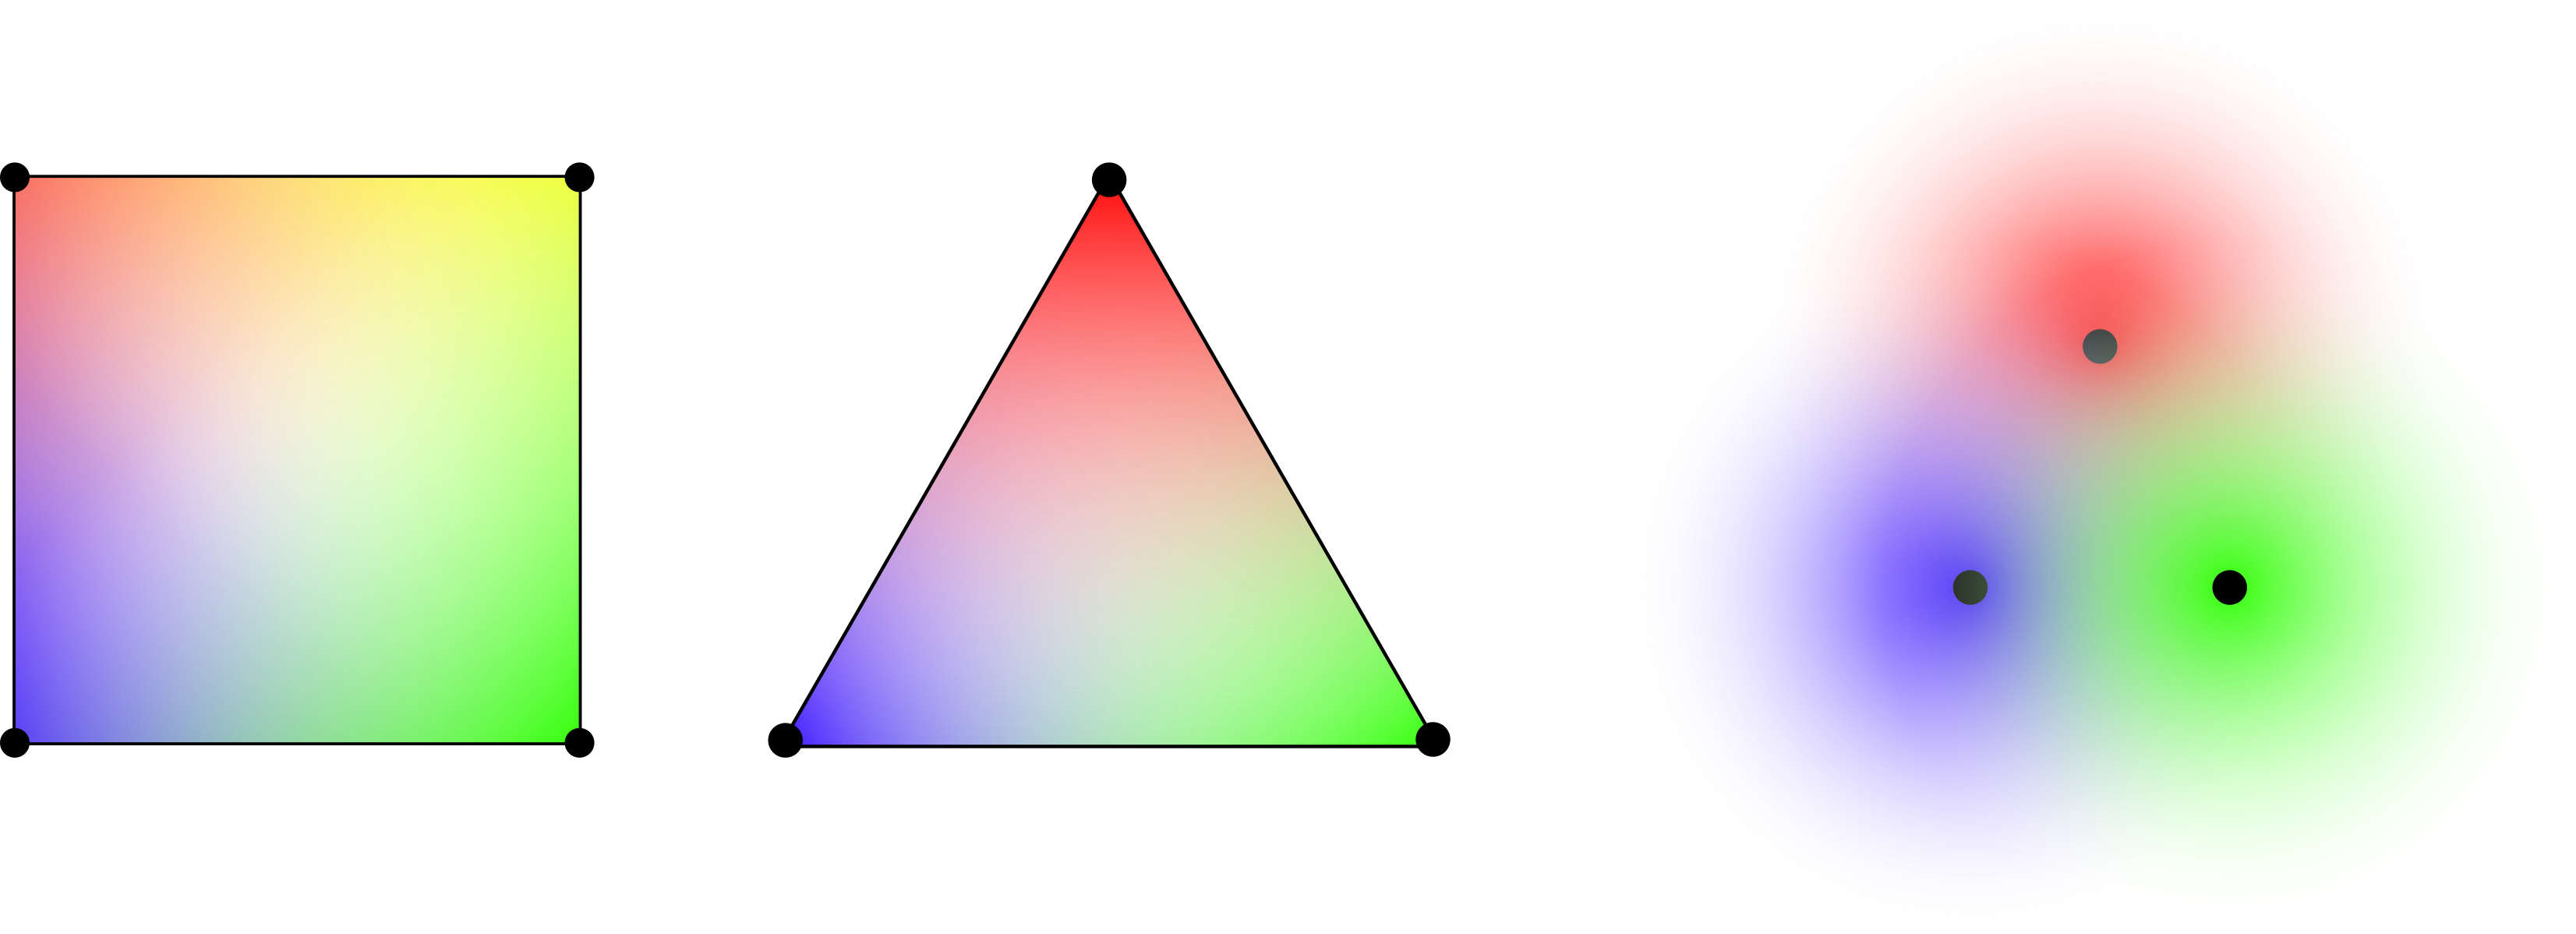
\includegraphics[width=\linewidth]{images/continuum_mechanics/shapefunction.png}
	\caption[STAR mechanics: Shape functions]{\label{fig:shapefunction} 
		Three examples of shape functions. 
		Each color represents the shape function associated to one sample point(black circle) carrying the degrees of freedom. 
		On the left, shape functions for trilinear interpolation are illustrated. 
		In the middle, barycentric shape functions are illustrated. 
		On the right, kernel-based shape functions that are used in SPH and MLS interpolation are illustrated.}
\end{figure}
\\
The choice of the interpolation method mainly depends on how the material samples have been distributed. 
For a sampling based on cartesian grid, trilinear interpolation is often used, for instance in Eulerian simulations~\cite{Bridson2008}. 
For unstructured triangle meshes, linear interpolation with barycentric weights is the most popular choice to simulate elastic solids~\cite{Muller2008}.
For mesh-less samplings, the two most common interpolation methods are SPH and MLS.
SPH interpolation has been used to simulate a wide range of phenomena from fluid~\cite{Desbrun1999} to elastic solids~\cite{Becker2009}.
MLS has been introduced by M\"{u}ller et al. to simulate elastic and plastic deformations~\cite{Muller2004:melting}.
It was later extended to solids fracture by Pauly et al.~\cite{Pauly2005} and interactive cutting by Steinemann et al.~\cite{Steinemann2009}.
Both methods use a cubic kernel as weights and require a dense sampling of the object.
\\
Of course, mesh-based and mesh-less methods can be combined to get the best of both worlds.
In this case, two interpolation methods are used, one for the mesh-based side and one for the mesh-less side.
We refer the reader to the recent \emph{SIGGRAPH} course on the material point method~\cite{Jiang2016}.
In this course, existing hybrid models are compared and the interpolation methods to transfer data from one representation  to another are described.
\\
A common drawback of the methods mentioned above it that they require a dense sampling. In Chapter~\ref{chap:cutting}, we will detail the Voronoi-based interpolation method used in the frame-based model, which allows to use a sparse sampling and thus reduce the computational time.

\subparagraph{Spatial Integration}

Over the simulation, different physical quantities such as density or internal forces, need to be integrated over the domain. 
There is need for a quadrature rule. 
Many exist, most of the time the simple midpoint rule is chosen (see Figure~\ref{fig:spatialIntegration}). 
\begin{figure}[!h]
	\centering
	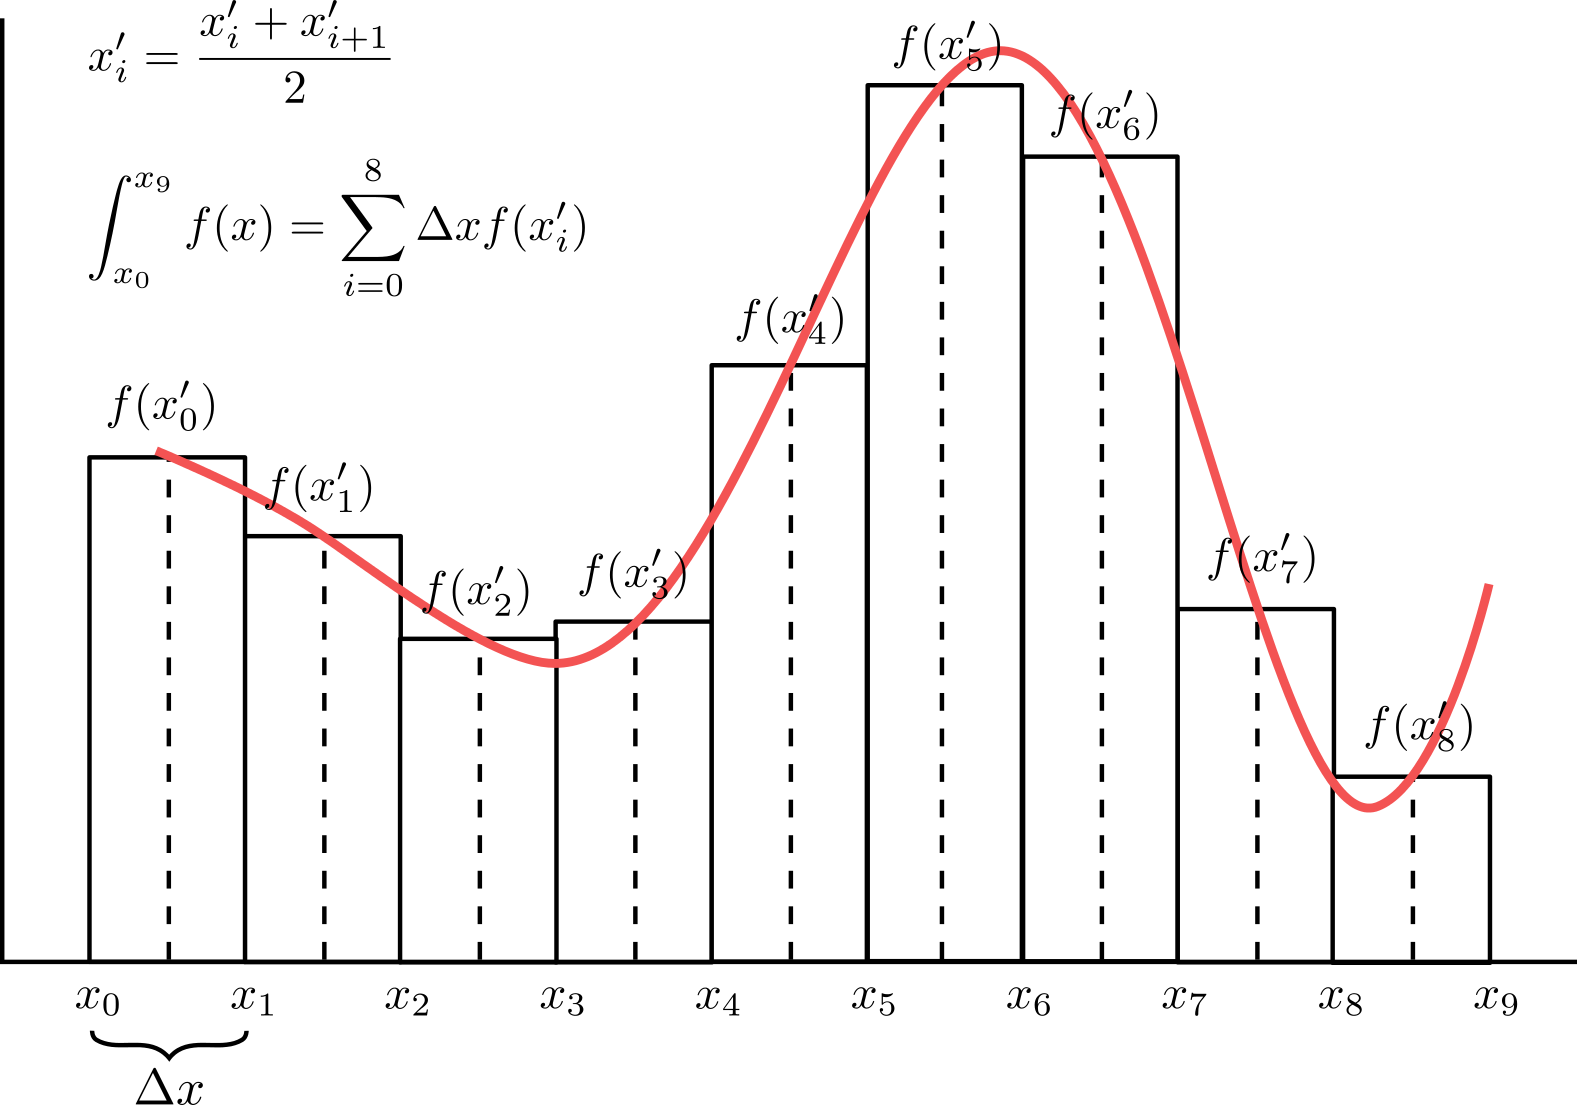
\includegraphics[width=\linewidth]{images/continuum_mechanics/spatialIntegration.png}
	\caption[STAR mechanics: Spatial integration]{\label{fig:spatialIntegration} Illustration of the midpoint rule for a one dimensional function. The integration domain is partitioned into uniform regions $\left[x_{i}, x_{i+1}\right]$, an integration point $x'_{i}$ is sampled at the center of each partition and the function is evaluated at the location of the integration points.}
\end{figure}
\\
The domain is decomposed in a set of partitions, where each partition has an associated volume $V_{i}$. 
"Mid"-Points $\mathbf{x}_{i}$ are sampled at the center of each partition.
They are called \emph{integration points}. 
Then the integral of a function $f$ over a domain $\Omega$ is approximated by:
\begin{equation}
\label{eq:midpointRule}
\int_{\Omega} f(x)dv \simeq \sum_{i} V_{i}f(\mathbf{x}_{i})
\end{equation}
In mesh-based methods, it is common to consider one integration point at the center of each element and integrate over the volume of the element.
In mesh-less methods, when the sampling is dense, integration points are often co-located with the material samples and integrated over their associated volume. 
However, when the sampling is sparse, an independent sampling of integration points can be used to get a finer integration.
This is the case in the frame-based method that will be described in Section~\ref{subsubsec:framebased}.

\paragraph{Time integration}

Once physical quantities are spatially integrated, they can be integrated over time. 
\begin{equation}
\label{eq:timeIntegration1}
\displaystyle
\int_{t_{n}}^{t_{n+1}}
m \frac{d\mathbf{v}}{dt} dt
=
\int_{t_{n}}^{t_{n+1}}\mathbf{f} dt
\end{equation}
In the following we assume an uniform discretization of the time where the time step is noted $\Delta t$.
Adaptive discretization of the time will be presented in Section~\ref{sec t adaptivity}.
Many integrations schemes can be used. 
Most of them can be explained simply by the Taylor expansion.
\begin{equation}
\label{eq:taylorExpansion}
\displaystyle
f(x) = \sum_{k=0}^{n}\frac{\left(x-a\right)^{k}}{k!}f^{(k)}(a) + \int_{a}^{x}\frac{\left(x-t\right)^{n}}{n!}f^{(n+1)}(t)dt
\end{equation}
Applied to equation (\ref{eq:timeIntegration1}), this gives:
\begin{equation}
\label{eq:timeIntegration2}
\displaystyle
\mathbf{v}(t_{n+1}) = \mathbf{v}(t_{n}) + \int_{t_{n}}^{t_{n+1}}\frac{1}{m}\frac{d\mathbf{v}}{dt} dt
\end{equation}
This expression can be further expanded in order to get more accurate results. 
In Computer Graphics, this is the most used expansion. 
Generally, the integral term is computed with the rectangle quadrature rule.
For a left rectangle method, we get an explicit integration of the velocity:
\begin{equation}
\label{eq:explicitIntegration}
\mathbf{v}(t_{n+1}) = \mathbf{v}(t_{n}) + \left(t_{n+1}-t_{n}\right) \frac{\mathbf{f}(t_{n})}{m}
\end{equation}
For a right rectangle method, we get an implicit integration of the velocity:
\begin{equation}
\label{eq:implicitIntegration}
\mathbf{v}(t_{n+1}) = \mathbf{v}(t_{n}) + \left(t_{n+1}-t_{n}\right) \frac{\mathbf{f}(t_{n+1})}{m}
\end{equation}
The same rule applies for the integration of other physical quantities. In a Lagrangian system, both velocity and position needs to be integrated. There are mainly three different schemes that are used in Computer Graphics: forward Euler, symplectic Euler and backward Euler.
\begin{figure}[!ht]
	\centering
	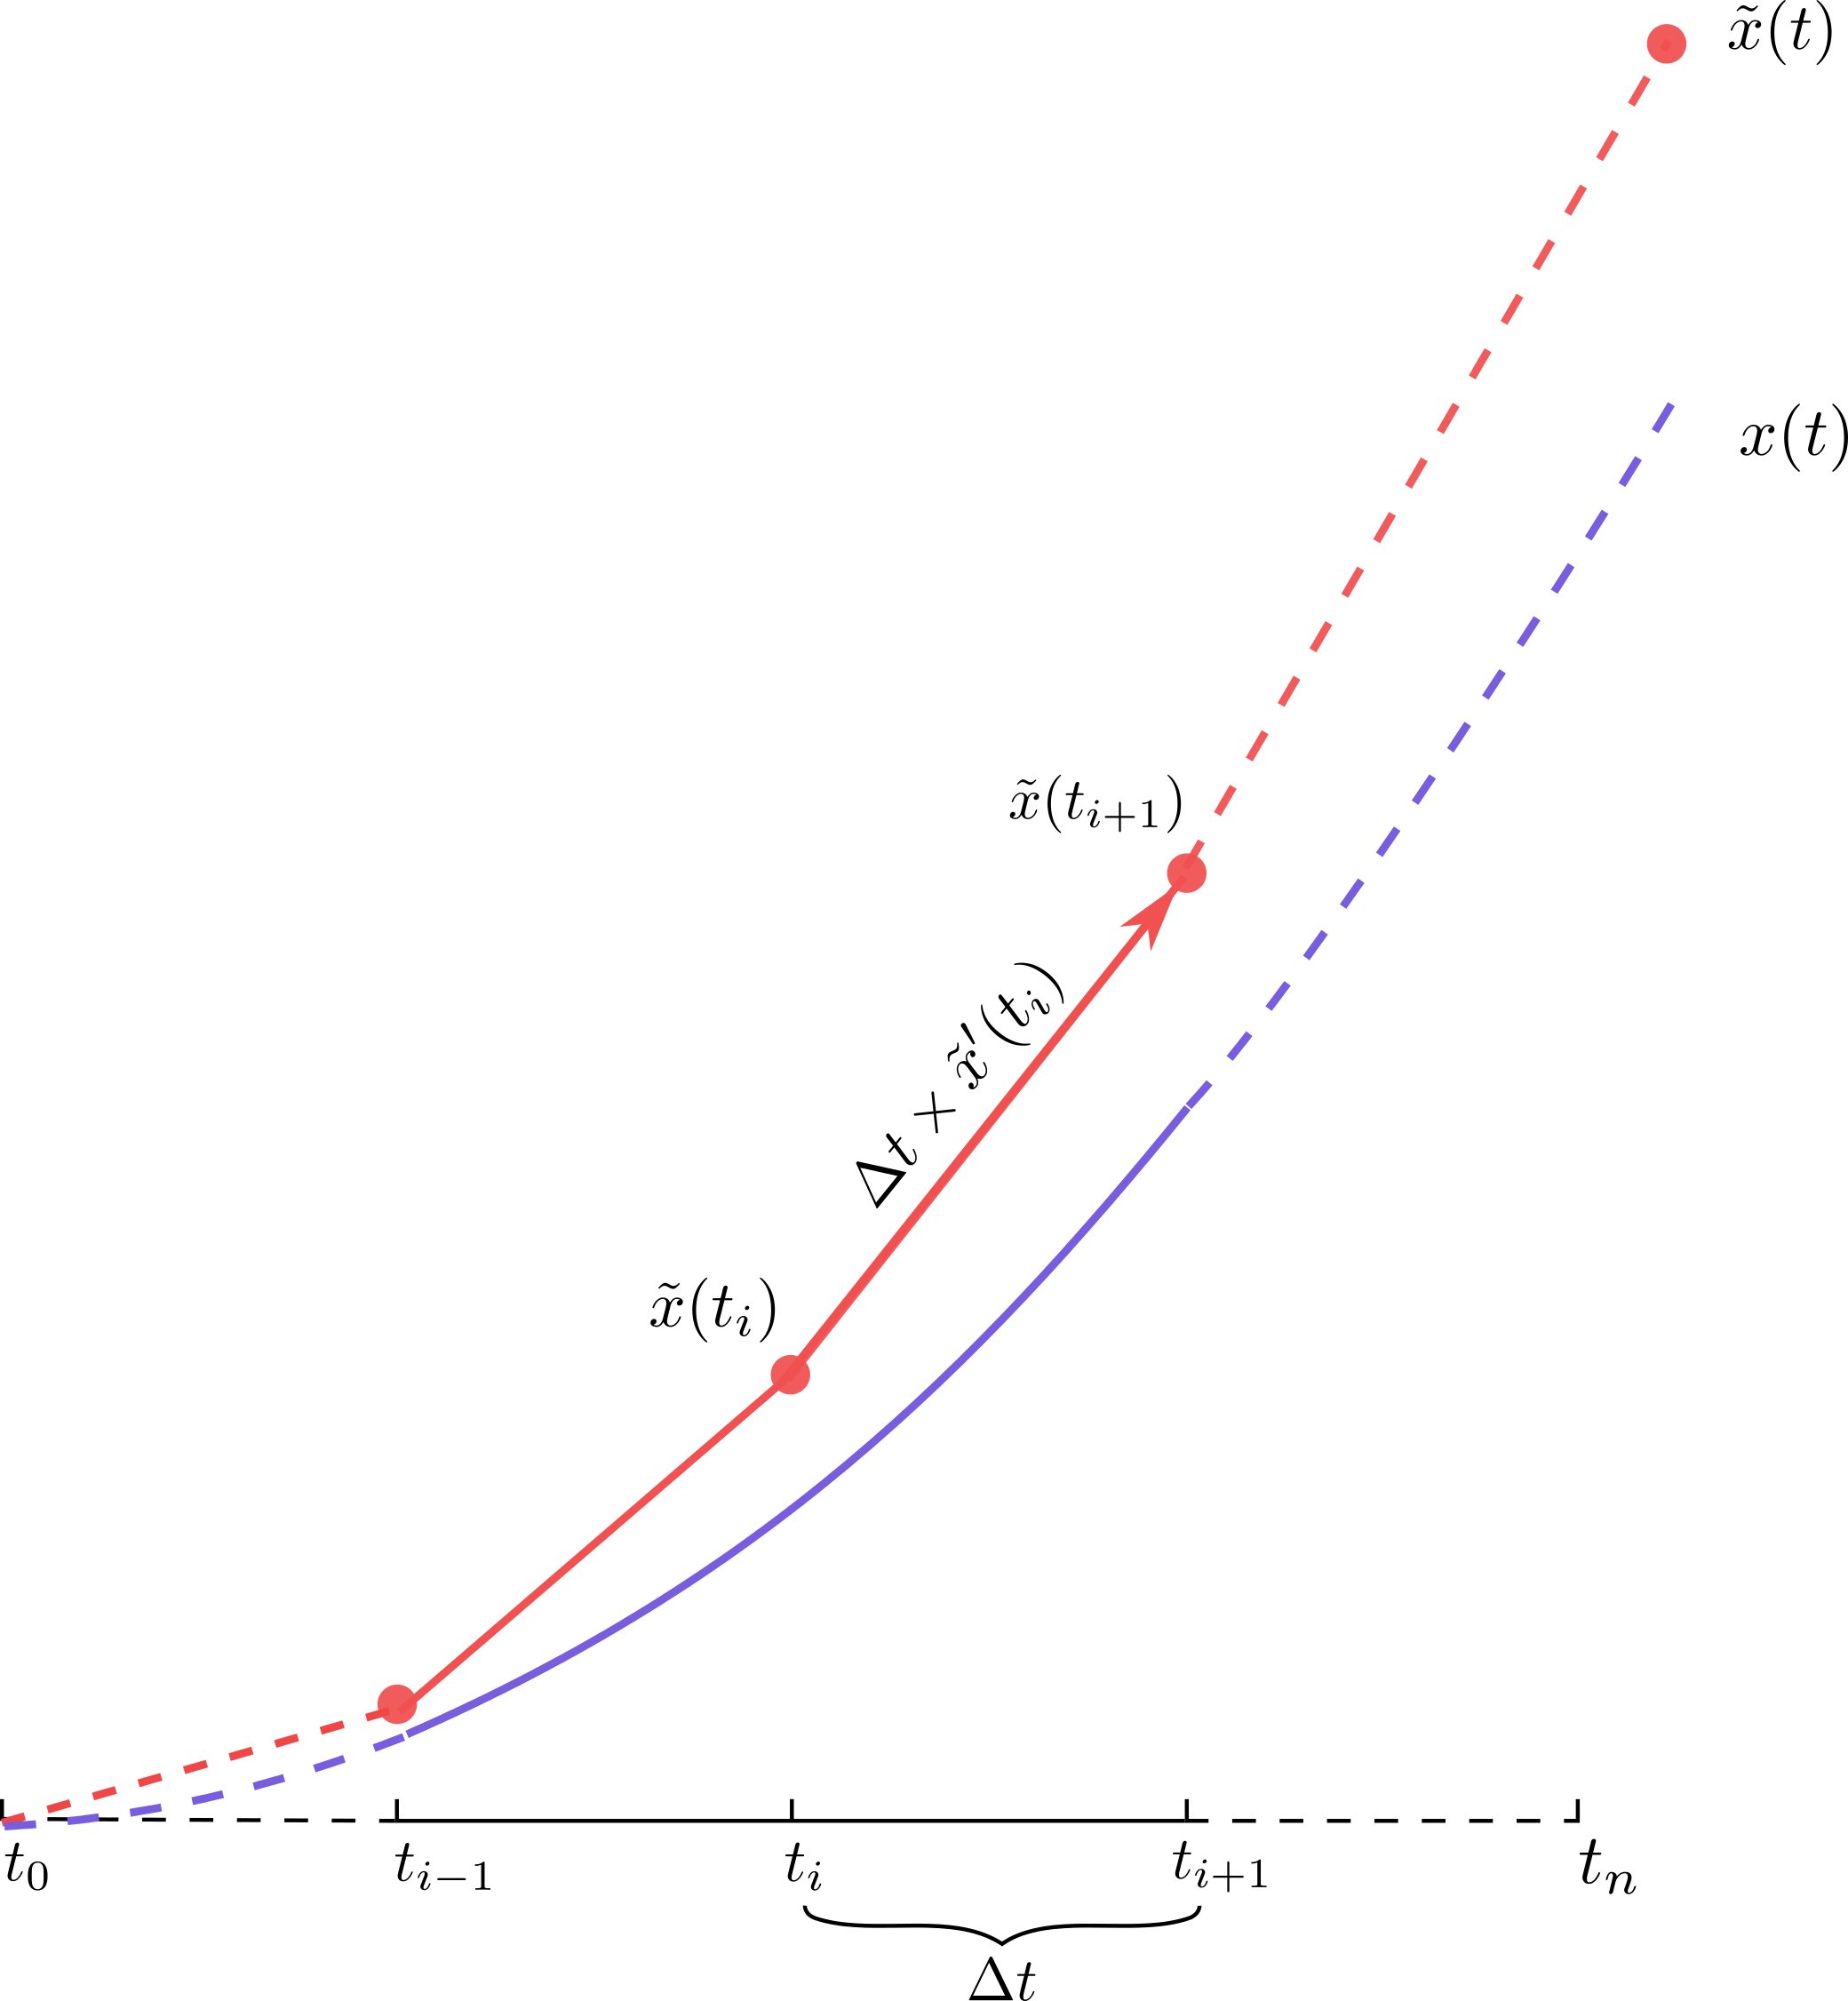
\includegraphics[scale=0.6]{images/continuum_mechanics/timeIntegration.png}
	\caption[STAR mechanics: Temporal integration]{\label{fig:timeIntegration} 
		Illustration of a 1D forward Euler time integration. 
		$x(t)$ describes the solution and $x'(t)$ describes the numerical approximation.}
\end{figure}
Forward Euler is the explicit integration of both position and velocity,
Figure~\ref{fig:timeIntegration} illustrates the integration of position in 1D:
\begin{equation}
\label{eq:explicitEuler}
\begin{array}{l}
\displaystyle \mathbf{x}(t+\Delta t) = \mathbf{x}(t) + \Delta t \mathbf{v}(t) \\ \\
\displaystyle \mathbf{v}(t+\Delta t) = \mathbf{v}(t) + \Delta t \frac{\mathbf{f(t)}}{m}(t)
\end{array}
\end{equation}

Symplectic Euler is the explicit integration of velocity and implicit integration of position:
\begin{equation}
\label{eq:symplecticEuler}
\begin{array}{l}
\displaystyle \mathbf{v}(t+\Delta t) = \mathbf{v}(t) + \Delta t \frac{\mathbf{f}(t)}{m} \\ \\
\displaystyle \mathbf{x}(t+\Delta t) = \mathbf{x}(t) + \Delta t \mathbf{v}(t+\Delta t)
\end{array}
\end{equation}

Backward Euler is the implicit integration of both position and velocity
\begin{equation}
\label{eq:backwardEuler}
\begin{array}{ll}
\displaystyle \mathbf{v}(t+\Delta t) = \mathbf{v}(t) + \Delta t \frac{\mathbf{f}(t)}{m}(t+\Delta t) \\ \\
\displaystyle \mathbf{x}(t+\Delta t) = \mathbf{x}(t) + \Delta t \mathbf{v}(t+\Delta t)
\end{array}
\end{equation}

Forward and symplectic Euler are among the easiest integration schemes. 
They are cheap and easy to implement. 
However, stability is guaranteed for a restricted range of time steps. 
Backward Euler is more expensive as it requires the solution an equation. 
However unconditional stability is guaranteed which means that large time steps can be used resulting in a significant speed-up of the simulation. This speed-up comes at the price of numerical damping which might be undesired.

A nice way to solve the non-linear equation of backward Euler is to expand the force expression in order to fall back to solving a linear system. There, efficient iterative methods such as the conjugate gradient can be used.

\subsection{Fluid mechanics}
\label{subsec:fluidMechanics}

\subsubsection{Constitutive Law}

A fluid mainly reacts to pressure and viscosity and thus the constitutive law can be written as:
\begin{equation}
\label{eq:fluidConstitutiveLaw}
\sigma = -pI + \eta \left( \nabla \mathbf{v} + \nabla \mathbf{v}^{T} \right)
\end{equation}

Then we have:
\begin{equation}
\nabla \cdot \sigma = \nabla \cdot \left( -pI + \eta \left( \nabla \mathbf{v} + \nabla \mathbf{v}^{T} \right) \right) = -\nabla p + \Delta \mathbf{v}
\end{equation}

Additionally, the fluid might be incompressible, such as water, which means that the mass should not vary over time. In this case, the conservation of mass can be rewritten as:
\begin{equation}
\nabla \cdot \mathbf{v} = 0
\end{equation}

Finally, by injecting equation~(\ref{eq:fluidConstitutiveLaw}) in equation~(\ref{eq:volumetricMomentumConservation}), this gives us Navier-Stokes equations for an incompressible fluid:

\begin{equation}
\label{eq:navierStokes}
\left\lbrace
\begin{array}{ll}
\displaystyle \int_{\mathcal{V}} \rho \frac{d}{dt} \mathbf{v}(t,x) dv = 
\displaystyle \int_{\mathcal{V}} \rho \mathbf{g} -\nabla p + \eta \Delta \mathbf{v} dv \\ \\
\displaystyle
\nabla. \mathbf{v} = 0
\end{array}
\right.
\end{equation}

\subsubsection{Smoothed-Particles Hydrodynamics model}
\label{subsubsec:starSPH}
Smoothed-Particles Hydrodynamics (SPH) is an interpolation method that can be used to approximate Navier-Stokes equations in a Lagrangian way. SPH was initially proposed by Monaghan et al.~\cite{Monaghan1992} and introduced in graphics by Desbrun et al.~\cite{Desbrun1999}.
The fluid is discretized into particles which represent small volumes of the whole fluid and each quantity is interpolated using SPH.

\paragraph{SPH interpolation}
The interpolation of a function $f$ at a position $\mathbf{x}$ is :
\begin{equation}
f(\mathbf{x}) = \int_{V} f(\mathbf{x'})W(\mathbf{x}-\mathbf{x'}, h)dx'
\end{equation}
where $W$ is a function called \emph{kernel} and $h$ is a smoothing radius, also called length scale, which represents the support of $W$.

If the fluid is discretized into particles with a mass $m$, a density $\rho$ and a volume $V$, then we can discretize the SPH interpolation as:
\begin{equation}
f(\mathbf{x}) = \sum_{p} f(\mathbf{x}_{p})V_{p} W(\mathbf{x}-\mathbf{x_{p}},h) = \sum_{p} f(\mathbf{x}_{p})\frac{m_{p}}{\rho_{p}} W(\mathbf{x}-\mathbf{x_{p}},h)
\end{equation}

\begin{equation}
\label{eq:sphFunction}
f(\mathbf{x}) = \sum_{p} f(\mathbf{x}_{p})\frac{m_{p}}{\rho_{p}} W(\mathbf{x}-\mathbf{x_{p}},h)
\end{equation}

Derivatives can be computed and discretized the same way:
\begin{equation}
D^{\alpha} f(\mathbf{x}) = \int_{\mathcal{V}} f(\mathbf{x'}) D^{\alpha} W(\mathbf{x}-\mathbf{x'}, h)dx'
\end{equation}

\begin{equation}
\label{eq:sphDerivative}
D^{\alpha} f(\mathbf{x})= \sum_{p} f(\mathbf{x}_{p})\frac{m_{p}}{\rho_{p}} D^{\alpha} W(\mathbf{x}-\mathbf{x_{p}},h)
\end{equation}

However, for first derivatives, the approximation above does not vanish if $f$ is a constant function. 
A quick way to ensure this expected property is to use an arbitrary differentiable function $\Phi$ and to rewrite the derivative using the derivative of a product :
\begin{equation}
\label{eq:hackSPH}
\nabla f(x) = \frac{1}{\Phi}\left(\nabla (f \Phi) - f \nabla \Phi \right)
\end{equation}
Then, if $f$ is constant, $\nabla f = 0$.
In practice, the density $\rho$ is used for $\Phi$ most of the time.

\paragraph{How to choose the kernel}
The properties of $W$ can vary with respect to the properties of the function to be interpolated. In general, $W$ meet the following properties:
\begin{itemize}
\item $W$ is normalized. Thus, constants are interpolated exactly.
\item $W$ has a compact support.
\begin{equation}
\parallel \mathbf{x} \parallel \geq h \rightarrow W(\mathbf{x},h) = 0 
\end{equation}
\begin{equation}
\int_{\mathcal{V}} W(\mathbf{x},h) dx = 1
\end{equation}
\item $W$ tends to the delta function when the length scale $h$ tends to $0$.
\begin{equation}
\lim_{h \rightarrow 0} W(x,h) = \delta(x)
\end{equation}
\item $W$ should be symmetric to enforce invariance under rotation
\begin{equation}
W(-x,h) = W(x,h)
\end{equation}
\item Depending on the function to interpolate the kernel should be positive to prevent unphysical interpolated value.
\begin{equation}
W \geq 0
\end{equation}
\end{itemize}

In practice, the cubic kernel from Monaghan~\cite{Monaghan1992} illustrated in Figure~\ref{fig:cubicKernel} is a good choice.
This is the kernel we use in Chapter~\ref{chap:arps}.

\begin{figure}[!ht]
	\centering
	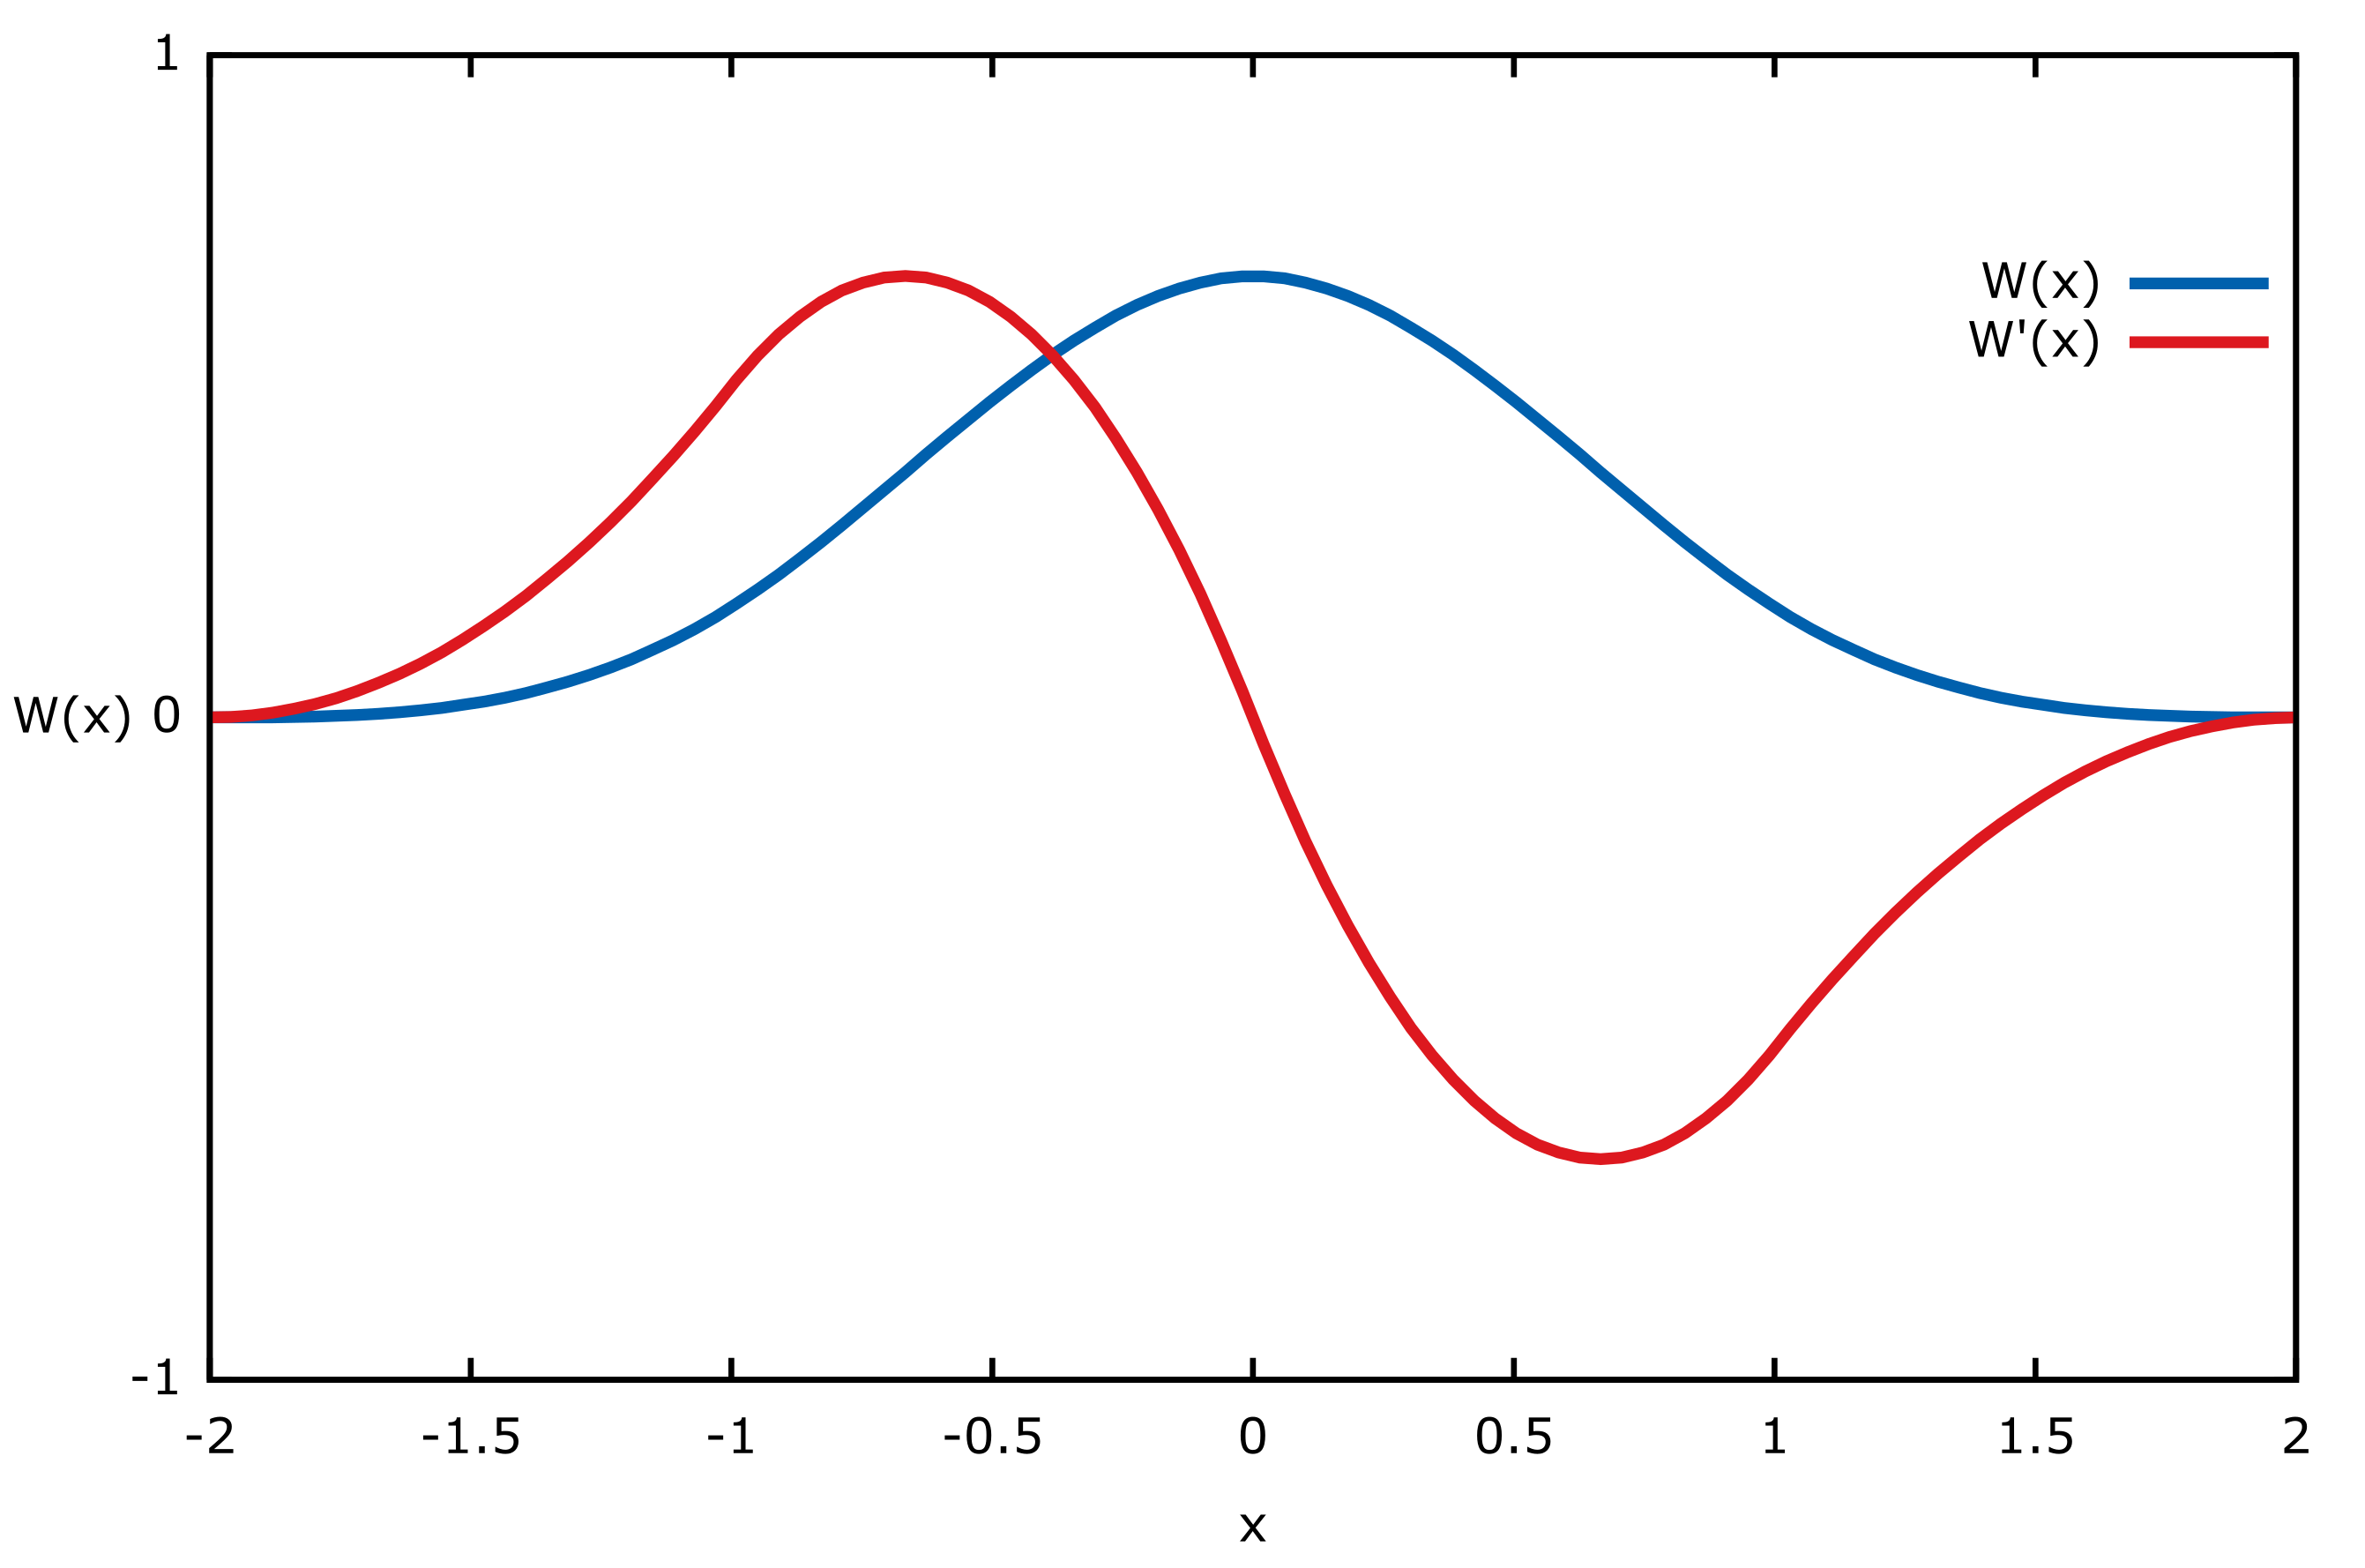
\includegraphics[scale=0.6]{images/continuum_mechanics/cubicKernel.png}
	\caption[STAR mechanics: Cubic kernel]{\label{fig:cubicKernel}
		Illustration of the 1D cubic kernel used by Monaghan et al.~\cite{Monaghan1992} and its derivative.
    In this image, the length scale $h$ is equal to $1$ and the kernel has a $2h$ support radius.}
\end{figure}

\paragraph{Application to Navier-Stokes equations}

In computer graphics, the SPH model is commonly used to approximate the Navier-Stokes equations (Equation~\ref{eq:navierStokes}).
In the following, we discretize each term of these equations for a particle $i$ using the SPH model.
\\ \\
The density of a particle $i$ can be approximated using Equation~(\ref{eq:sphFunction}):

\begin{equation}
\label{eq:densitySPH}
\rho_{i} = \sum_{j} m_{j}W(\mathbf{x_{i}}-\mathbf{x_{j}},h)
\end{equation}

For the pressure gradient, we can directly apply Equation~(\ref{eq:sphDerivative}):

\begin{equation}
\left(\nabla p\right)_{i} = \sum_{j} \frac{m_{j}}{\rho_{j}} p_{j} \nabla W(\mathbf{x_{i}}-\mathbf{x_{j}},h)
\end{equation}

However, the resulting pressure force between two particles $i$ and $j$ is not symmetric and therefore does not conserve linear and angular momentum:
\begin{equation}
\label{eq:nonSymmetricPressureForce}
\mathbf{f}^{pressure}_{ij} = \frac{m_{i}m_{j}}{\rho_{i}\rho_{j}}p_{j}\nabla W(\mathbf{x_{i}}-\mathbf{x_{j}},h)
\end{equation}

A symmetric version can be obtained by using equation~(\ref{eq:hackSPH}) with $\displaystyle \Phi = \frac{1}{\rho}$:

\begin{equation}
\label{eq:pressureGradientSPH}
\left(\nabla p\right)_{i} = 
\frac{1}{\rho_{i}}
\sum_{j} m_{j} \left( \frac{p_{i}}{\rho_{i}^{2}} + \frac{p_{j}}{\rho_{j}^{2}} \right) \nabla W(\mathbf{x_{i}}-\mathbf{x_{j}},h)
\end{equation}

Various techniques exist to compute pressure.
In Monaghan et al.~\cite{Monaghan1992} and Desbrun et al.~\cite{Desbrun1996}, a spring-like equation of state was used:
\begin{equation}
\label{eq:pressureSPH}
p_{i} = k\left(\rho_{i}-\rho_{0}\right)
\end{equation}
where $k$ is a stiffness parameter. 
Even though it is simple and cheap, high stiffness and very small time steps are required to get close to incompressibility.
Recently, new techniques were proposed to compute pressure so that the fluid would be incompressible while allowing the use of large time steps.
We do not detail these methods in this manuscript but refer the reader to the work of Ihmsen et al.~\cite{Ihmsen2014:IISPH} and Bender and Koschier~\cite{Bender2015}.
\\ \\
To compute viscosity forces, we could approximate the Laplacian of the velocity using Equation~(\ref{eq:sphDerivative}):

\begin{equation}
\left(\Delta \mathbf{v}\right)_{i} = \sum_{j} \frac{m_{j}}{\rho_{j}} \mathbf{v}_{j} \Delta W(\mathbf{x_{i}}-\mathbf{x_{j}},h)
\end{equation}

Same as for the pressure gradient, this would result in a non-symmetric force:

\begin{equation}
\label{eq:nonSymmetricViscosityForce}
\mathbf{f}^{viscosity}_{ij} = \eta\frac{m_{i}m_{j}}{\rho_{i}\rho_{j}}\mathbf{v}_{j}\Delta W(\mathbf{x_{i}}-\mathbf{x_{j}},h)
\end{equation}

To obtain symmetric inter-particle forces, we can use a technique similar to Equation~(\ref{eq:hackSPH}) to approximate the Laplacian of a function $f$ using an arbitrary twice differentiable function $\Phi$:

\begin{equation}
\label{eq:hackSPH2}
\Delta f = 
\frac{1}{\Phi}
\left( \Delta \left( f\rho \right) - 2 \nabla f \nabla \phi - f \Delta \phi \right)
\end{equation}

By using $\Phi=\rho$ and assuming that the density is constant, which should be the case in theory, we can obtain a new expression that will result in symmetric inter-particle forces:

\begin{equation}
\left(\Delta \mathbf{v}\right)_{i} = \frac{1}{\rho_{i}}\sum_{j} m_{j} \left( \mathbf{v}_{j}-\mathbf{v}_{i}\right) \Delta W(\mathbf{x_{i}}-\mathbf{x_{j}},h)
\end{equation}

However, in practice, density is not constant and the evaluation of the second derivative of the kernel is sensitive to particles sampling, which makes this expression inadequate.
The evaluation of viscosity is still an area of research and various solutions exist depending whether it is important or not in the phenomena that we want to simulate.
For liquids exhibiting complex viscous behaviors such as coiling or buckling, implicit formulations were recently proposed by Peer et al.~\cite{Peer2015} and Takahashi et al.~\cite{Takahashi2015}.
In practice, the evaluation of the Laplacian is not accurate. 
As we do not seek to simulate this kind of behavior, we can stick to a gradient-based formulation of viscosity which was proposed by Monaghan~\cite{Monaghan2005}.

\begin{equation}
\label{eq:velocityLaplacianSPH}
\left(\Delta \mathbf{v}\right)_{i} = 
\frac{1}{\rho_{i}}
\sum_{j} m_{j} \Pi_{ij} \nabla W(\mathbf{x_{i}}-\mathbf{x_{j}},h)
\end{equation}

where 

\begin{equation}
    \Pi_{ij} = -\frac{2hc_{s}}{\rho_{i}+\rho_{j}}\frac{\mathbf{v}_{ij}^{T}\mathbf{x}_{ij}}{\vert \mathbf{x}_{ij} \vert^{2} + \epsilon h^{2}}
\end{equation}
and $c_{s}$ is the speed of sound in the media and $\epsilon$ is a numerical constant to avoid singularities.
In practice, $\epsilon=0.01$ works well.
\\ \\
Finally, we have all the ingredients to write a discretized version of Navier-Stokes equations for one particle $i$:

\begin{equation}
    \displaystyle m_{i}\frac{d}{dt}\mathbf{v}_{i}(t) = m_{i}\mathbf{g} - \frac{m_{i}}{\rho_{i}}(\nabla p)_{i} + \eta\frac{m_{i}}{\rho_{i}}\left(\Delta \mathbf{v}\right)_{i}
\end{equation}

This equation can now be discretized in time and integrated. 
In practice, the Euler symplectic integrator is often used:

\begin{equation}
\begin{array}{ll}
\displaystyle \mathbf{v}_{i}(t+\Delta t) = \mathbf{v}_{i}(t) + \Delta t \frac{d}{dt}\mathbf{v}_{i}(t) \\ \\
\displaystyle \mathbf{x}_{i}(t+\Delta t) = \mathbf{x}_{i}(t) + \Delta t \mathbf{v}_{i}(t+\Delta t)
\end{array}
\end{equation}

We described the key ingredient of the SPH model and how to use them to discretize Navier-Stokes equations. 
There is not enough space to cover the exciting challenges related to the building of a full SPH simulator. 
For a robust handling of static and dynamic boundaries, a surface tension model and an efficient surface reconstruction pipeline, we refer to the work of Akinci et al.~\cite{Akinci2012b, Akinci2013, Akinci2012a}.  
For a state of the art of optimization techniques for SPH, we refer the reader to the work of Ihmsen et al.~\cite{Ihmsen2011:ParallelSPH}. 
For other references related to the handling of viscosity, multiphase simulations and other problems, the state of the art report on SPH by Ihmsen et al.~\cite{Ihmsen2014:STAR} is a safe starting point.

\subsection{Solid mechanics}
\label{subsec:solidMechanics}

\begin{figure}[!ht]
\centering
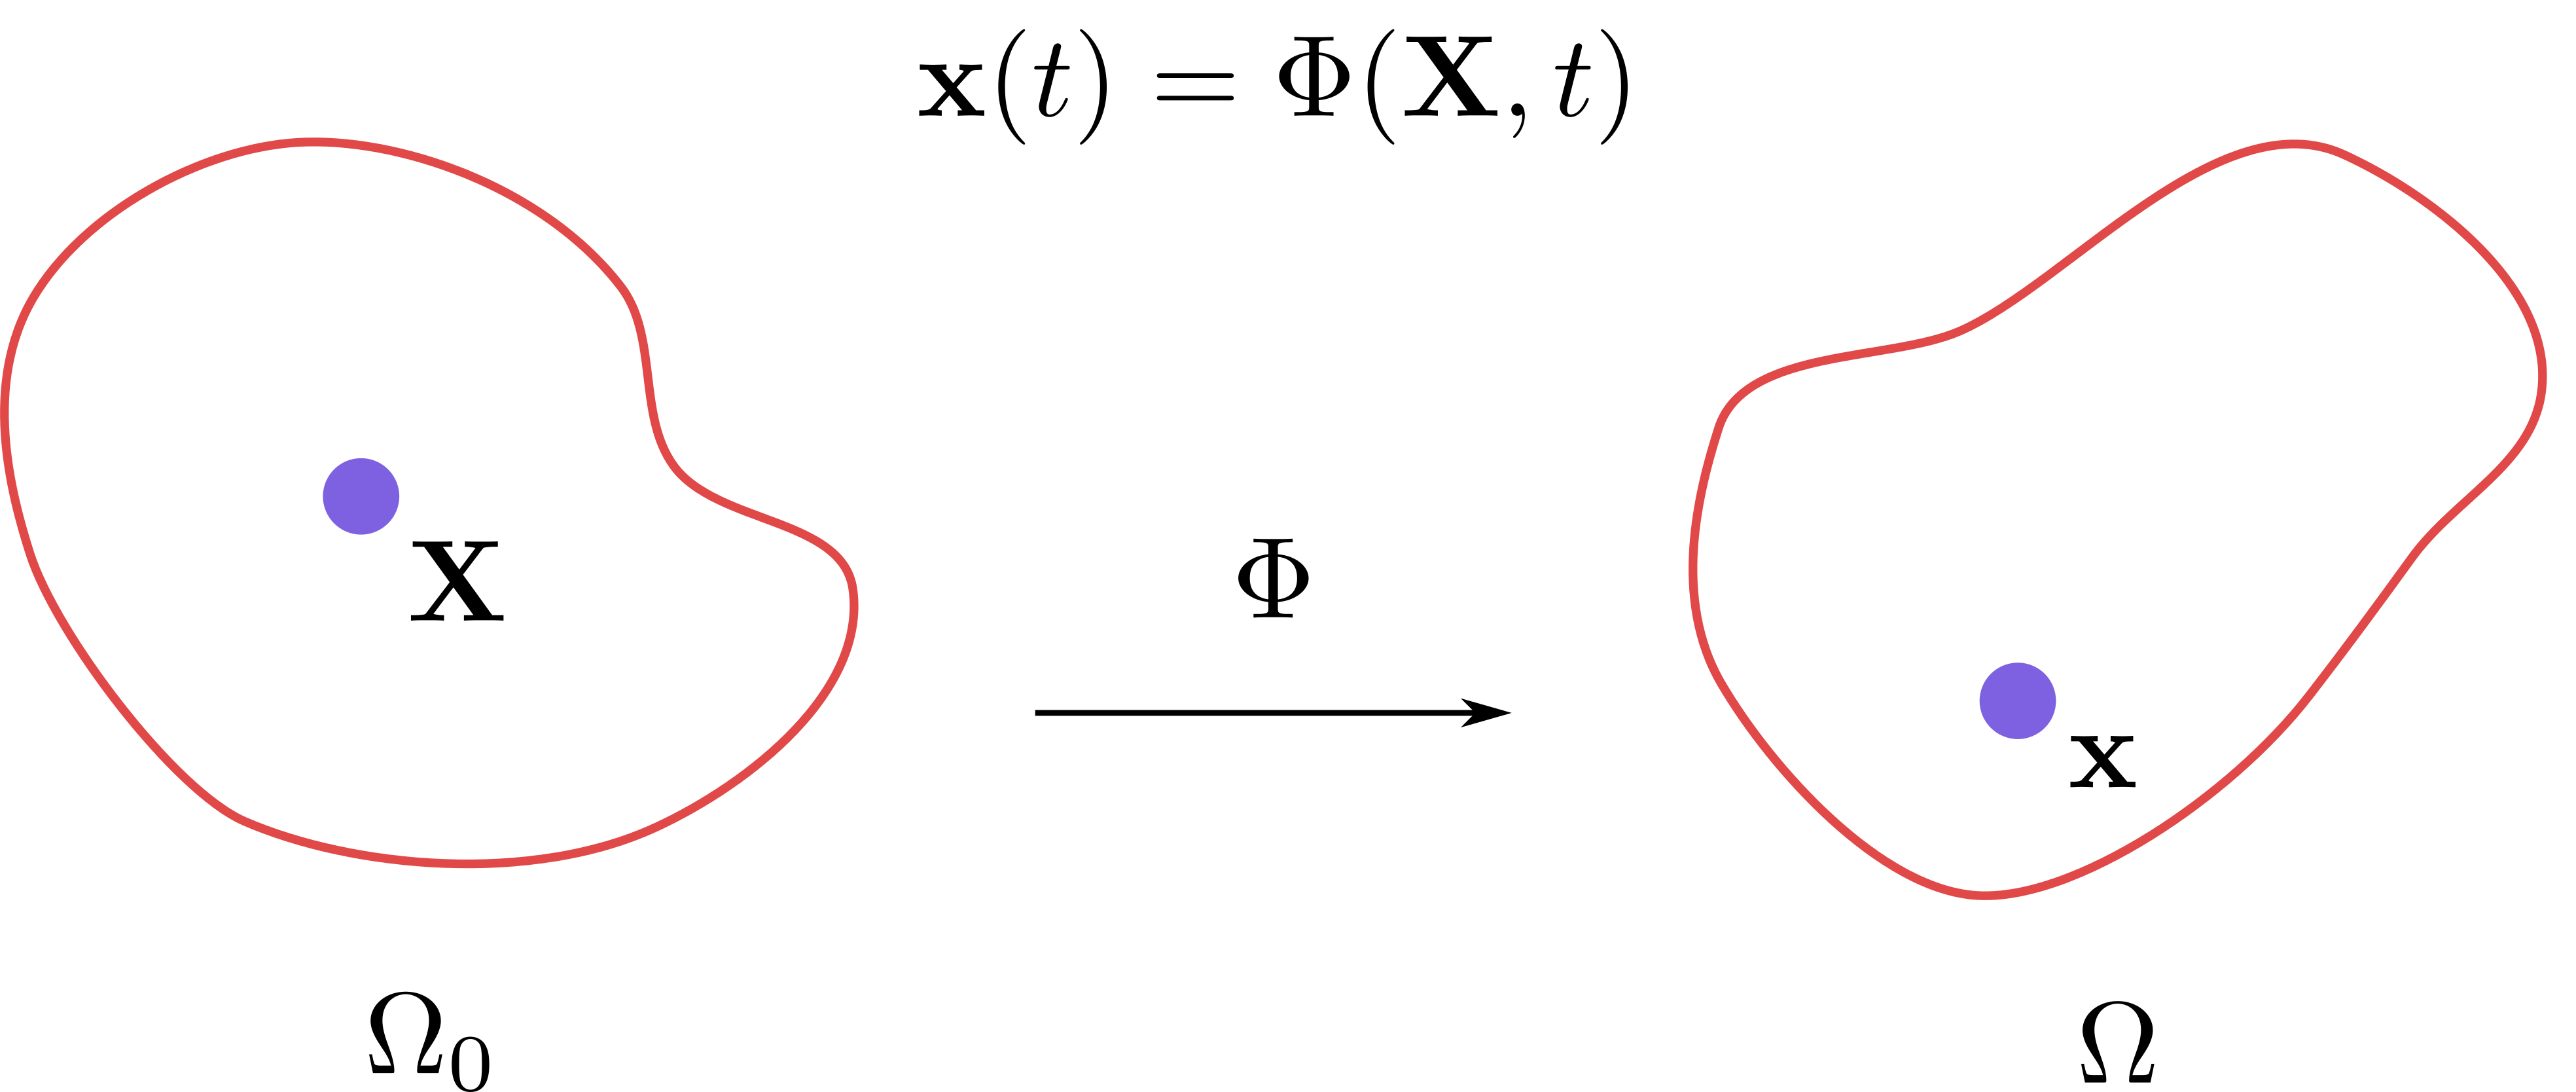
\includegraphics[scale=0.4]{./images/continuum_mechanics/displacementField.png}
\caption[STAR mechanics: Displacement field]{\label{fig:displacementField}
 The displacement field $\Phi$ maps each point $\mathbf{X}$ from the rest configuration $\Omega_{0}$ to a point $\mathbf{x}$ in the deformed configuration $\Omega$.}
\end{figure}

In this section, we focus on the simulation of elastic objects. When submitted to external forces, an elastic object reacts so that it comes back to its rest shape. In contrast with fluids, internal forces are history dependent, they depend on how much the object deformed compared to its rest shape. It becomes crucial to be able to describe the deformation of an object in order to express its reaction. 

The deformation is modeled by a mapping $\Phi$ between the undeformed configuration $\Omega_{0}$ and the deformed configuration $\Omega$ (see Figure~\ref{fig:displacementField}). $\Phi$ is called the \emph{displacement field}.
\begin{equation}
\begin{array}{lllll}
\Phi & : & \Omega_{0} & \longrightarrow & \Omega \\
	 &  & \mathbf{X} & \longrightarrow & \mathbf{x}
\end{array}
\end{equation}
where $\mathbf{X}$ is a point in the undeformed configuration and $\mathbf{x}=\Phi(\mathbf{X})$ is the mapped point into the deformed configuration.

The deformation gradient $\displaystyle F = \frac{\partial \Phi}{\partial \mathbf{X}}$ describes the local state subject to rigid and/or deformable displacement with respect to the undeformed configuration. 
The strain tensor $\epsilon$ measures the deformation.
Multiple strain measures have been proposed, Green-Lagrange strain can be used for instance: $\displaystyle \epsilon = \frac{1}{2}\left(F^{T}F - I\right)$. 
Or its linearized version, the Cauchy strain $\displaystyle \epsilon = \frac{1}{2}\left( F + F^{T} \right)-I$.

The displacement field, deformation gradient and strain tensor are the main components of the constitutive law that relates the deformation to the material properties of the object.

\subsubsection{Constitutive Law}
In this section, we focus on elastic materials, i.e objects which tends to recover their rest configuration after a deformation.
For elastic materials, the stress tensor $\sigma$ can be described using constitutive density energy $\Psi$ that is derived with respect to the strain tensor $\epsilon$:

\begin{equation}
\label{eq:constitutiveLaw}
\sigma = \frac{\partial \Psi}{\partial \epsilon}
\end{equation}

Different forms of energy exist. For a classical Hookean material, the density energy is
\begin{equation}
\Psi = \frac{1}{2}H\epsilon^{2}
\end{equation}

which gives the following stress tensor
\begin{equation}
\sigma = H\epsilon
\end{equation}

$H$ is called the stiffness tensor and is a $3\times3\times3\times3$ tensor. 
For isotropic materials, the number of material parameters can be reduced to two, the Young's modulus $E$ and the Poisson's ratio $\nu$. 
These parameters respectively describes the resistance of the object to extension and to shearing.
Moreover, the strain and stress tensor are symmetric which allows to simplify the constitutive law:
\begin{equation}
\sigma = 
\begin{bmatrix}
\sigma_{11} \\
\sigma_{22} \\
\sigma_{33} \\
\sigma_{23} \\
\sigma_{13} \\
\sigma_{12}
\end{bmatrix}
=
\tilde{H}
\begin{bmatrix}
\epsilon_{11} \\
\epsilon_{22} \\
\epsilon_{33} \\
2\epsilon_{23} \\
2\epsilon_{13} \\
2\epsilon_{12}
\end{bmatrix}
\end{equation}

where

\begin{equation}
\tilde{H} =
\frac{E}{\left(1+\nu\right)\left(1-2\nu\right)}
\begin{bmatrix}
1-\nu & \nu & \nu & 0 & 0 & 0 \\ 
\nu & 1-\nu & \nu & 0 & 0 & 0 \\
\nu & \nu & 1-\nu & 0 & 0 & 0 \\
0 & 0 & 0 & \frac{1-2\nu}{2} & 0 & 0 \\
0 & 0 & 0 & 0 & \frac{1-2\nu}{2} & 0 \\
0 & 0 & 0 & 0 & 0 & \frac{1-2\nu}{2} \\
\end{bmatrix}
\end{equation}

Instead of computing internal forces as the divergence of the stress, they can be computed as the derivative of the density energy with respect to the degrees of freedom:
\begin{equation}
\label{eq:internalForces}
\mathbf{f} = -\int_{\mathcal{V}} \frac{\partial \Psi}{\partial \mathbf{x}}^{T} dv
\end{equation}

\subsubsection{Frame-based model}
\label{subsubsec:framebased}
The frame-based model was introduced by Gilles et al.~\cite{Gilles2011} to simulate deformable objects. In contrast to other deformable models, it allows to simulate complex object with very few degrees of freedom and to handle heterogeneous materials easily \cite{Faure2011}. 
Additionally, this work formalized the concept of multi-layer physical framework. In the following, we first describe what is a multi-layer framework, illustrate it in the case of the frame-based model. 
Then we detail a standard choice for the different components of the frame-based model: degrees of freedom, interpolation and integration. As in the previous section, this section is a high level overview. 
Detailing collision detection and response processes and giving a more accurate formulation of viscosity via the strain rate are out of the scope of this chapter.

\paragraph{A multi-layer physical framework}
 
\begin{figure}[!ht]
\centering
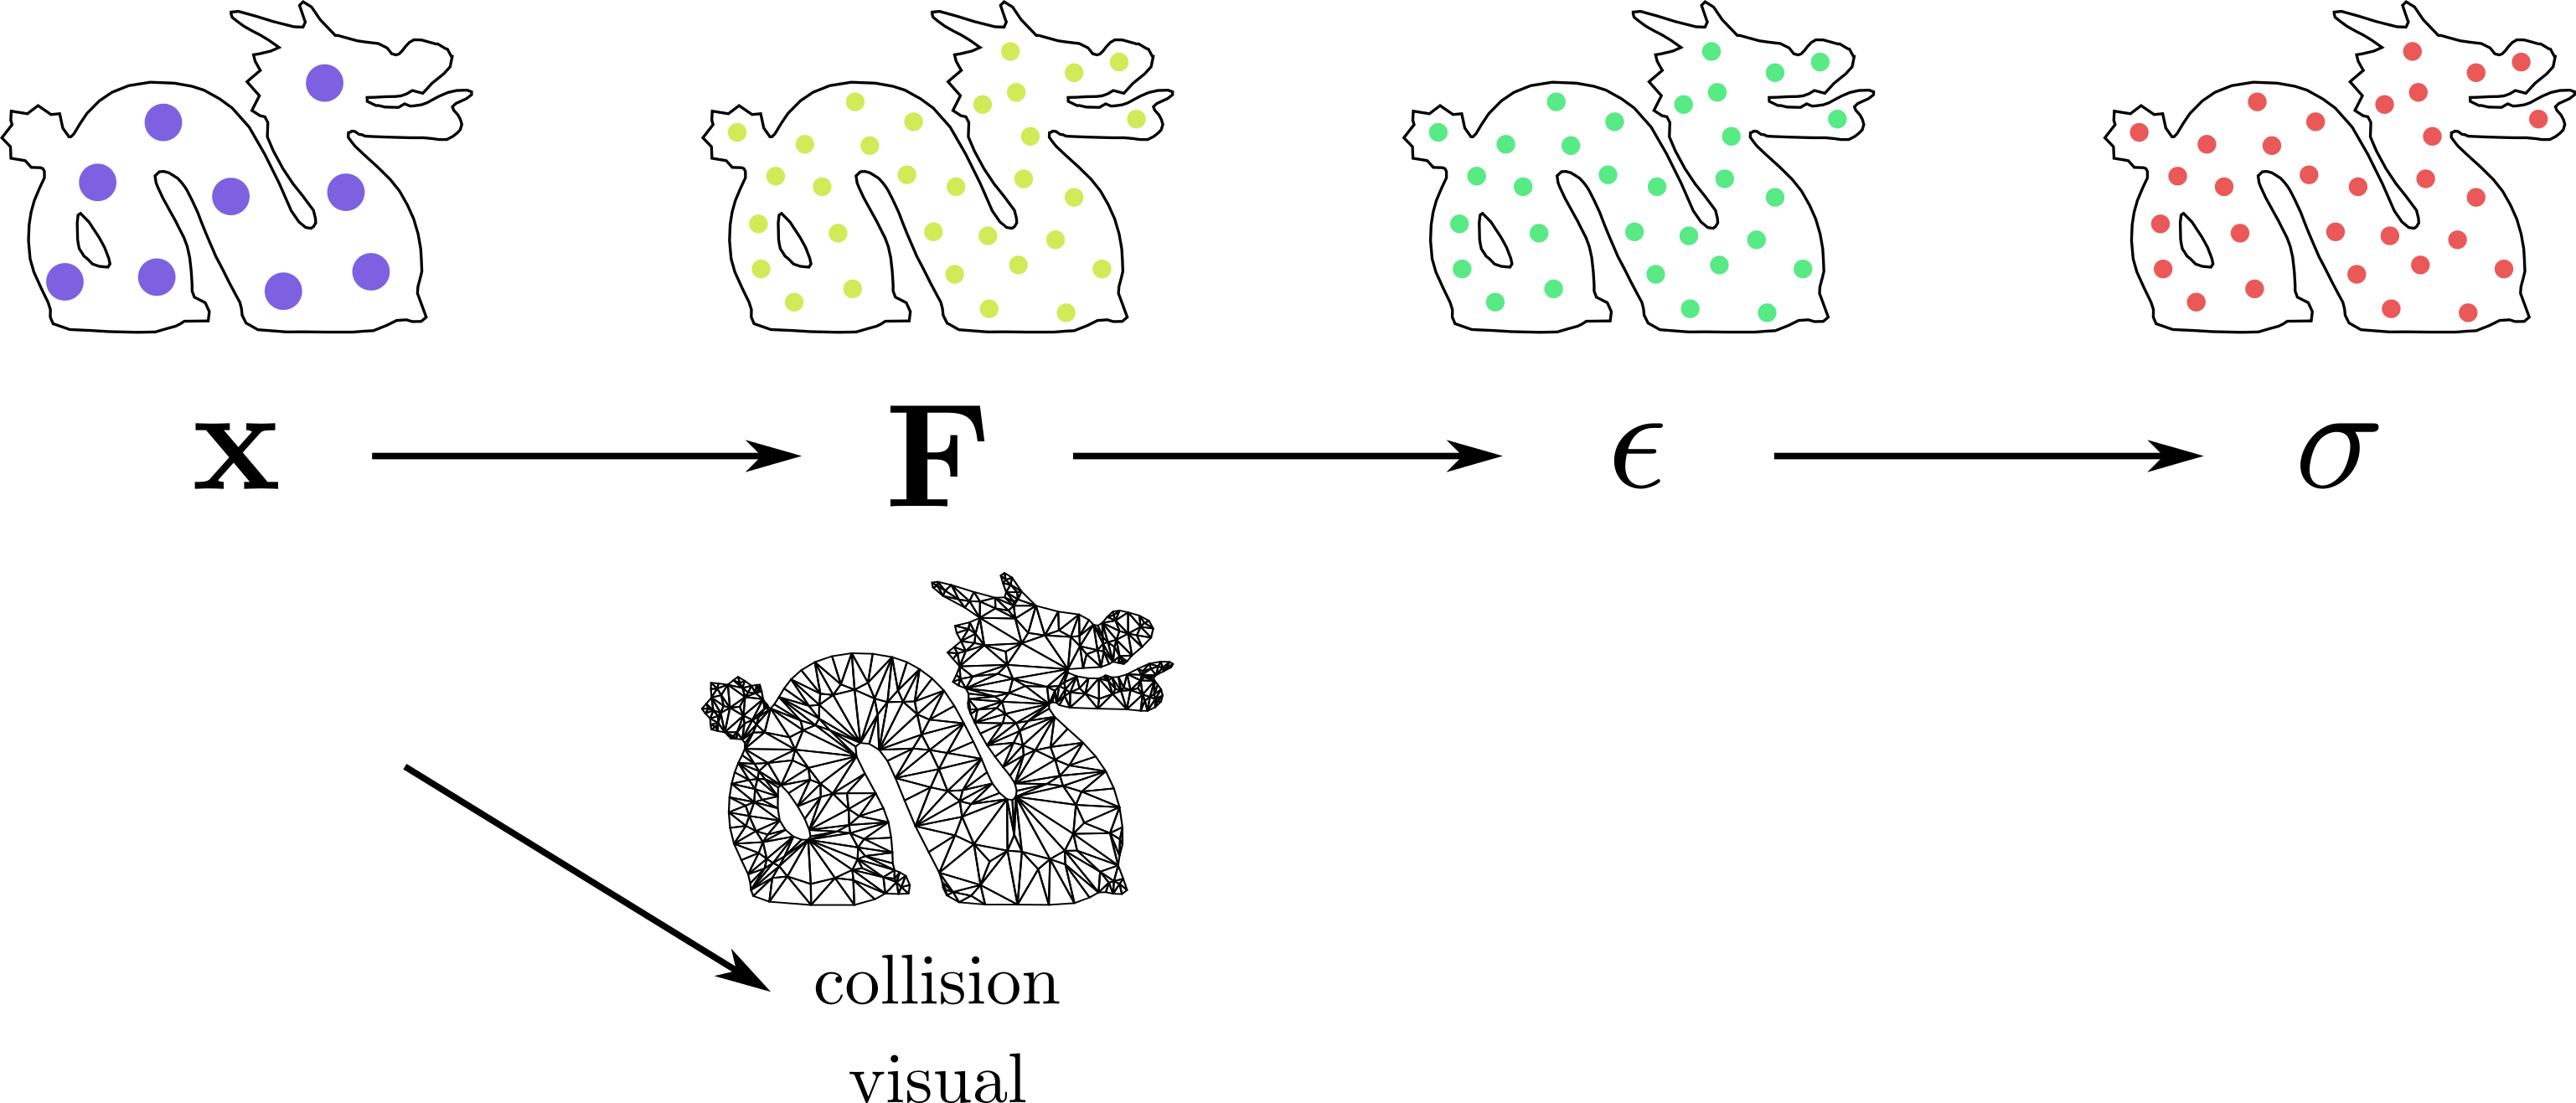
\includegraphics[scale=0.6]{./images/continuum_mechanics/multiLayeredFramework.png}
\caption[STAR mechanics: Multi-layer framework]{\label{fig:multiLayerFramework} Each component of the simulation is isolated and communicates with other components through mappings. By doing so, the framework allows fast prototyping and comparison of a wide range of deformable models.}
\end{figure}

Most of the time, the different components of a physics-based model are described as a monolithic framework: degrees of freedom, interpolation, integration and constitutive law are put together in one formula which computes the forces applied on the degrees of freedom. On one hand, this provides a compact and implementation-friendly expression. It also suits the short format of scientific article. On the other hand, it requires assumptions on each component and make it hard to distinguish what should be changed in order to integrate collisions, to embed a visual model or to test variations of the initial model.

An interesting alternative is to build a multi-layer framework where each component of a physics-based model represents a layer which is able to communicate with other layers through mappings. 
The framework has then a great modularity, as different components can be re-used and mixed. A direct consequence is the ease at prototyping. 
State of the art methods can be implemented in hours instead of days. 
Comparisons of different models is much easier. 
Also, it provides a way to control the granularity of a simulation, as each layer can be discretized at its own resolution, this allows for an easier repartition of resources and computational tasks.

In their work, Gilles et al. \cite{Gilles2011} proposed such an alternative by decomposing the computation of force using the derivation chain rule:
\begin{equation}
\label{eq:forceChainRule}
\displaystyle \mathbf{f} = -\int_{V} \left(\frac{\partial \Psi}{\partial \mathbf{x}}\right)^{T} dv
=
-\int_{V} \left(\frac{\partial F}{\partial \mathbf{x}}\right)^{T}
\left(\frac{\partial \epsilon}{\partial F}\right)^{T}
\left(\frac{\partial \Psi}{\partial \epsilon}\right)^{T} dv
\end{equation}
The three different layers are now visible: the degrees of freedom, the deformation gradient, the strain tensor and the constitutive density energy.
Moreover, we can distinguish the Jacobian of the mappings that link degrees of freedom to deformation gradient and deformation gradient to strain.
Notice that the derivative of the constitutive density energy with respect to strain is actually the stress tensor presented in Equation~(\ref{eq:constitutiveLaw}.

Using this modular representation offers three main advantages: 
First, layers and mappings can be implemented separately thus providing a great deal of modularity;
Secondly, it is straightforward to have a sampling of degrees of freedom different from the sampling of integration points.
Thus, multi-resolution strategies can easily be integrated. 
For instance, we might want a small number of degrees of freedom to have a small computational time during the solving of dynamics while computing accurate deformation gradient, strain and stress which requires a dense sampling of integration points.
Additionally, embedding techniques, used to display a fine visual model or to handles collision with a coarse representation, fits well in this framework.

In the case of the frame-based method, there are two additional layers, one for embedding a visual model and one for handling collisions. 
Both communicate with the degrees of freedom through a mapping which is the displacement field (see Figure~\ref{fig:multiLayerFramework}).

\paragraph{Degrees of freedom}
The object is uniformly sampled with affine frames as degrees of freedom. An affine frame $T=(A,\mathbf{t})$ represents $12$ degree of freedoms, $3$ for translation $\mathbf{t}$, $9$ for the matrix $A$ combining rotation, scaling and shearing. 
Affine frames are expressed with respect to an initial configuration ~$T_{0} = \left(A_{0}, \mathbf{t}_{0}\right)$.

\paragraph{Interpolation}
Linear blend skinning is used to interpolate the displacement field and other quantities of the simulation. A deformed position $\mathbf{x}$ can be interpolated as a weighted sum of the affine transformations applied to the rest position $\mathbf{x}_{0}$.

\begin{equation}
\label{eq:frameBasedDisplacementField}
\begin{array}{l}
\displaystyle \mathbf{x} = \Phi(\mathbf{x}_{0}) = \sum_{i} w_{i}(\mathbf{x}_{0})\left(\mathbf{t}_{i}+A_{i}\mathbf{x}_{0}^{rel}\right) \\
\displaystyle \mathbf{x}_{0}^{rel} = A_{0}^{-1}\left( \mathbf{x}_{0} - \mathbf{t}_{0} \right)
\end{array}
\end{equation}

where $\mathbf{x}_{0}^{rel}$ is the relative position of $x_{0}$ in the frame defined by $T_{0}$ and $w_{i}$ is the shape function associated to the frame $i$.

Different weights can be used. Three properties are important in order to represent a physical behavior. 
First, the shape function should linearly decrease with respect to distance in the material. 
Otherwise, the deformation will not be uniform with respect to the distance from the frame. 
Second, the shape function should be positive. 
Third, the weights should form a partition of unity. 
In practice, one can use either harmonic weights or Voronoi-based weights.
In Chapter~\ref{chap:cutting}), we will detail the computation of Voronoi-based weights and how to dynamically update them to take into account topological changes.

From the description of the displacement field (Equation~\ref{eq:frameBasedDisplacementField}), the deformation gradient can then be derived:
\begin{equation}
\displaystyle
F\left(\mathbf{x}\right) = \sum_{i} \frac{\partial \mathbf{x}}{\partial \mathbf{x}_{0}} =
\nabla w_{i}(\mathbf{x}_{0}) \left( \mathbf{t}_{i}+A_{i}\mathbf{x}_{0}^{rel}\right) + 
w_{i}\left( A_{i}A_{0}^{-1} \right)
\end{equation}

\paragraph{Spatial integration}

Any quadrature rule can be used. Here, for the sake of simplicity, we suppose that we use the midpoint rule briefly described in Figure~\ref{fig:spatialIntegration}. Thus, the integral of a function $f$ over the object states:
\begin{equation}
\displaystyle
\int_{V} f(\mathbf{x})  = \sum_{p} V_{p} f(\mathbf{x}_{p})
\end{equation}
where $p$ is an integration point and $V_{p}$ its associated volume.
\\ \\
From this quadrature rule, we can now formulate the computation of internal forces for one frame as:
\begin{equation}
\label{eq:frameForceComputation}
\displaystyle
\mathbf{f}_{i} =
- \sum_{p}
\left( \frac{\partial F}{\partial \mathbf{x}_{i}} \right)^{T}
\left( \frac{\partial \epsilon}{\partial F} \right)^{T}
\left( \frac{\partial \Psi}{\partial \mathbf{\epsilon}} \right)^{T} \left(\mathbf{x_{p}}\right) V_{p} 
\end{equation}
where $p$ is an integration point, $\mathbf{x}_{p}$ its position and $V_{p}$ its associated volume.

\paragraph{Temporal integration}

Assuming the mass matrix is lumped and that we use explicit Euler, the time integration of one frame $i$ is:
\begin{equation}
\displaystyle
\begin{pmatrix}
\mathbf{t}_{i}(t+\Delta t) \\
A_{i}(t+\Delta t)
\end{pmatrix} 
=
\begin{pmatrix}
\mathbf{t}_{i}(t) \\
A_{i}(t)
\end{pmatrix} 
+
\Delta t
M_{i}^{-1}
\mathbf{f}(t)
\end{equation}
where $M_{i}$ is the mass matrix of the frame $i$:
\begin{equation}
\label{eq:massMatrix}
M_{i} = \int_{V} w_{i}^{T} \rho w_{i} dv
\end{equation}
and $w_{i}$ is the shape function of the frame $i$.

\subsection{Conclusion on continuum mechanics}

In this section, we briefly presented the basics of continuum mechanics.
First, we described how to design equations of motion and which numerical tools are involved in their solving. 
Then, for fluids and solids mechanics, we mentioned their specificities and detailed a deformable model.
We illustrated the fact that continuum mechanics allows to automatically compute realistic motion from a wide range of phenomena.
This strength mainly explains why hand-made animations of physical phenomena have been replaced by physics-based animation.
However, realism comes with a high computational cost.
This cost may make large scale simulations intractable or prevent from simulating advanced phenomena in interactive context.
In the following section, we review adaptive models, a common approach to make simulations efficient.
